%%%%%%%%%%%%%%%%%%%%%%%%%%%%%%%%%%%%%%%%%
% Beamer Presentation
% LaTeX Template
% Version 1.0 (10/11/12)
%
% This template has been downloaded from:
% http://www.LaTeXTemplates.com
%
% License:
% CC BY-NC-SA 3.0 (http://creativecommons.org/licenses/by-nc-sa/3.0/)
%
%%%%%%%%%%%%%%%%%%%%%%%%%%%%%%%%%%%%%%%%%

%----------------------------------------------------------------------------------------
%	PACKAGES AND THEMES
%----------------------------------------------------------------------------------------

%%TO COMPILE AND GENERATE THE INDEX
%pdflatex TRUST_tutorial.tex
%makeindex TRUST_tutorial.idx
%pdflatex TRUST_tutorial.tex
%pdflatex TRUST_tutorial.tex

\documentclass[10pt]{beamer}

\mode<presentation> {

% The Beamer class comes with a number of default slide themes
% which change the colors and layouts of slides. Below this is a list
% of all the themes, uncomment each in turn to see what they look like.

%\usetheme{default}
%\usetheme{AnnArbor}
%\usetheme{Antibes}
%\usetheme{Bergen}
%\usetheme{Berkeley}
%\usetheme{Berlin}
%\usetheme{Boadilla}
\usetheme{CambridgeUS}
%\usetheme{Copenhagen}
%\usetheme{Darmstadt}
%\usetheme{Dresden}
%\usetheme{Frankfurt}
%\usetheme{Goettingen}
%\usetheme{Hannover}
%\usetheme{Ilmenau}
%\usetheme{JuanLesPins}
%\usetheme{Luebeck}
%\usetheme{Madrid}
%\usetheme{Malmoe}
%\usetheme{Marburg}
%\usetheme{Montpellier}
%\usetheme{PaloAlto}
%\usetheme{Pittsburgh}
%\usetheme{Rochester}
%\usetheme{Singapore}
%\usetheme{Szeged}
%\usetheme{Warsaw}

% As well as themes, the Beamer class has a number of color themes
% for any slide theme. Uncomment each of these in turn to see how it
% changes the colors of your current slide theme.

%\usecolortheme{albatross} % bleubleu
%\usecolortheme{beaver} % rouge
%\usecolortheme{beetle} % bleu/gris
%\usecolortheme{crane}  % jaune
%\usecolortheme{dolphin} % bleu
%\usecolortheme{dove}  % blanc
%\usecolortheme{fly} % gris
%\usecolortheme{lily} % bleu
%\usecolortheme{orchid} % bleu
%\usecolortheme{rose} % bleu
%\usecolortheme{seagull} % gris
%\usecolortheme{seahorse} % bleu pale
%\usecolortheme{whale} % bleu
%\usecolortheme{wolverine} % jaune/bleu

%\setbeamertemplate{footline} % To remove the footer line in all slides uncomment this line
%\setbeamertemplate{footline}[page number] % To replace the footer line in all slides with a simple slide count uncomment this line

%\setbeamertemplate{navigation symbols}{} % To remove the navigation symbols from the bottom of all slides uncomment this line

}

\usepackage{graphicx} % Allows including images
\usepackage{booktabs} % Allows the use of \toprule, \midrule and \bottomrule in tables
%\usepackage{multimedia} % for video
\definecolor{darkblue}{HTML}{3535b4}
\usepackage{multirow}
\usepackage{makeidx}
    \makeindex

\newenvironment{theindex}
 {\let\item\par
  %definitions for subitem etc
  }{}
\newcommand\indexspace{}

%----------------------------------------------------------------------------------------
%	TITLE PAGE
%----------------------------------------------------------------------------------------
%\title[Short title]{Long title}
\title[TRUST tutorial v1.7.1]{TRUST tutorial v1.7.1} % The short title appears at the bottom of every slide, the full title is only on the title page

%\author{John Smith} % Your name
\institute[CEA/DEN/DANS/DM2S/STMF] % Your institution as it will appear on the bottom of every slide, may be shorthand to save space
{
CEA Saclay \\ % Your institution for the title page
\medskip
\textit{triou@cea.fr} % Your email address
}
\date{\today} % Date, can be changed to a custom date






\begin{document}

%%%%%%%%%%%%%%%%%%%%%%%%%%%%%%%%%%%%%%%%%%%%%%%%%%%%%%%%%%%%%%%%%%%%%%%%
\begin{frame}
\titlepage % Print the title page as the first slide
\end{frame}
%%%%%%%%%%%%%%%%%%%%%%%%%%%%%%%%%%%%%%%%%%%%%%%%%%%%%%%%%%%%%%%%%%%%%%%%

%%%%%%%%%%%%%%%%%%%%%%%%%%%%%%%%%%%%%%%%%%%%%%%%%%%%%%%%%%%%%%%%%%%%%%%%
\begin{frame}
\frametitle{Overview} % Table of contents slide, comment this block out to remove it
%\tableofcontents[sectionstyle=show/show,subsectionstyle=hide/hide/hide ] 
\begin{columns}[c] 
\column{.45\textwidth}
\tableofcontents[sections={1-6}, hideallsubsections]
\column{.5\textwidth} 
\tableofcontents[sections={7-12}, hideallsubsections]
\end{columns}
% Throughout your presentation, if you choose to use \section{} and \subsection{} commands, these will automatically be printed on this slide as an overview of your presentation
\end{frame}
%%%%%%%%%%%%%%%%%%%%%%%%%%%%%%%%%%%%%%%%%%%%%%%%%%%%%%%%%%%%%%%%%%%%%%%%

%----------------------------------------------------------------------------------------
%	PRESENTATION SLIDES
%----------------------------------------------------------------------------------------

\section{Initialization}
%%%%%%%%%%%%%%%%%%%%%%%%%%%%%%%%%%%%%%%%%%%%%%%%%%%%%%%%%%%%%%%%%%%%%%%%
\begin{frame}
\frametitle{Initialization}
\begin{block}{}

\begin{itemize}
\item First, initialize the TRUST environment. On CEA Saclay PCs, TRUST versions are available with (e.g. X.Y.Z=1.7.1):\\
\vspace{0.2cm}
\textbf{source  /home/triou/env\_TRUST\_X.Y.Z\_patch.sh}
\vspace{0.5cm}

\item Second, several editors (vi, emacs, nedit) are configured to highlight TRUST keywords in the data files. If you prefer using \textbf{nedit}, please do the following:

    \begin{itemize}
    \item [$\circ$] Run \textbf{nedit}, and select Preferences $\rightarrow$ Save Defaults.
    \item [$\circ$] Then re-initialize the TRUST environment (cf first point), the message "nedit.rc updated" should appear.
    \end{itemize}
\end{itemize}

\end{block}
\end{frame}
%%%%%%%%%%%%%%%%%%%%%%%%%%%%%%%%%%%%%%%%%%%%%%%%%%%%%%%%%%%%%%%%%%%%%%%%



\section{Obstacle VDF}
\subsection{Obstacle: Sequentiel calculation}
%%%%%%%%%%%%%%%%%%%%%%%%%%%%%%%%%%%%%%%%%%%%%%%%%%%%%%%%%%%%%%%%%%%%%%%%
\begin{frame}
\begin{columns}[c] 
\column{.45\textwidth}
\tableofcontents[sections={1-6},currentsection, currentsubsection]
\column{.5\textwidth} 
\tableofcontents[sections={7-12},currentsection, currentsubsection]
\end{columns}
\end{frame}
%%%%%%%%%%%%%%%%%%%%%%%%%%%%%%%%%%%%%%%%%%%%%%%%%%%%%%%%%%%%%%%%%%%%%%%%
%%%%%%%%%%%%%%%%%%%%%%%%%%%%%%%%%%%%%%%%%%%%%%%%%%%%%%%%%%%%%%%%%%%%%%%%
\begin{frame}
\frametitle{Geometry}
\begin{block}{}

\begin{figure}
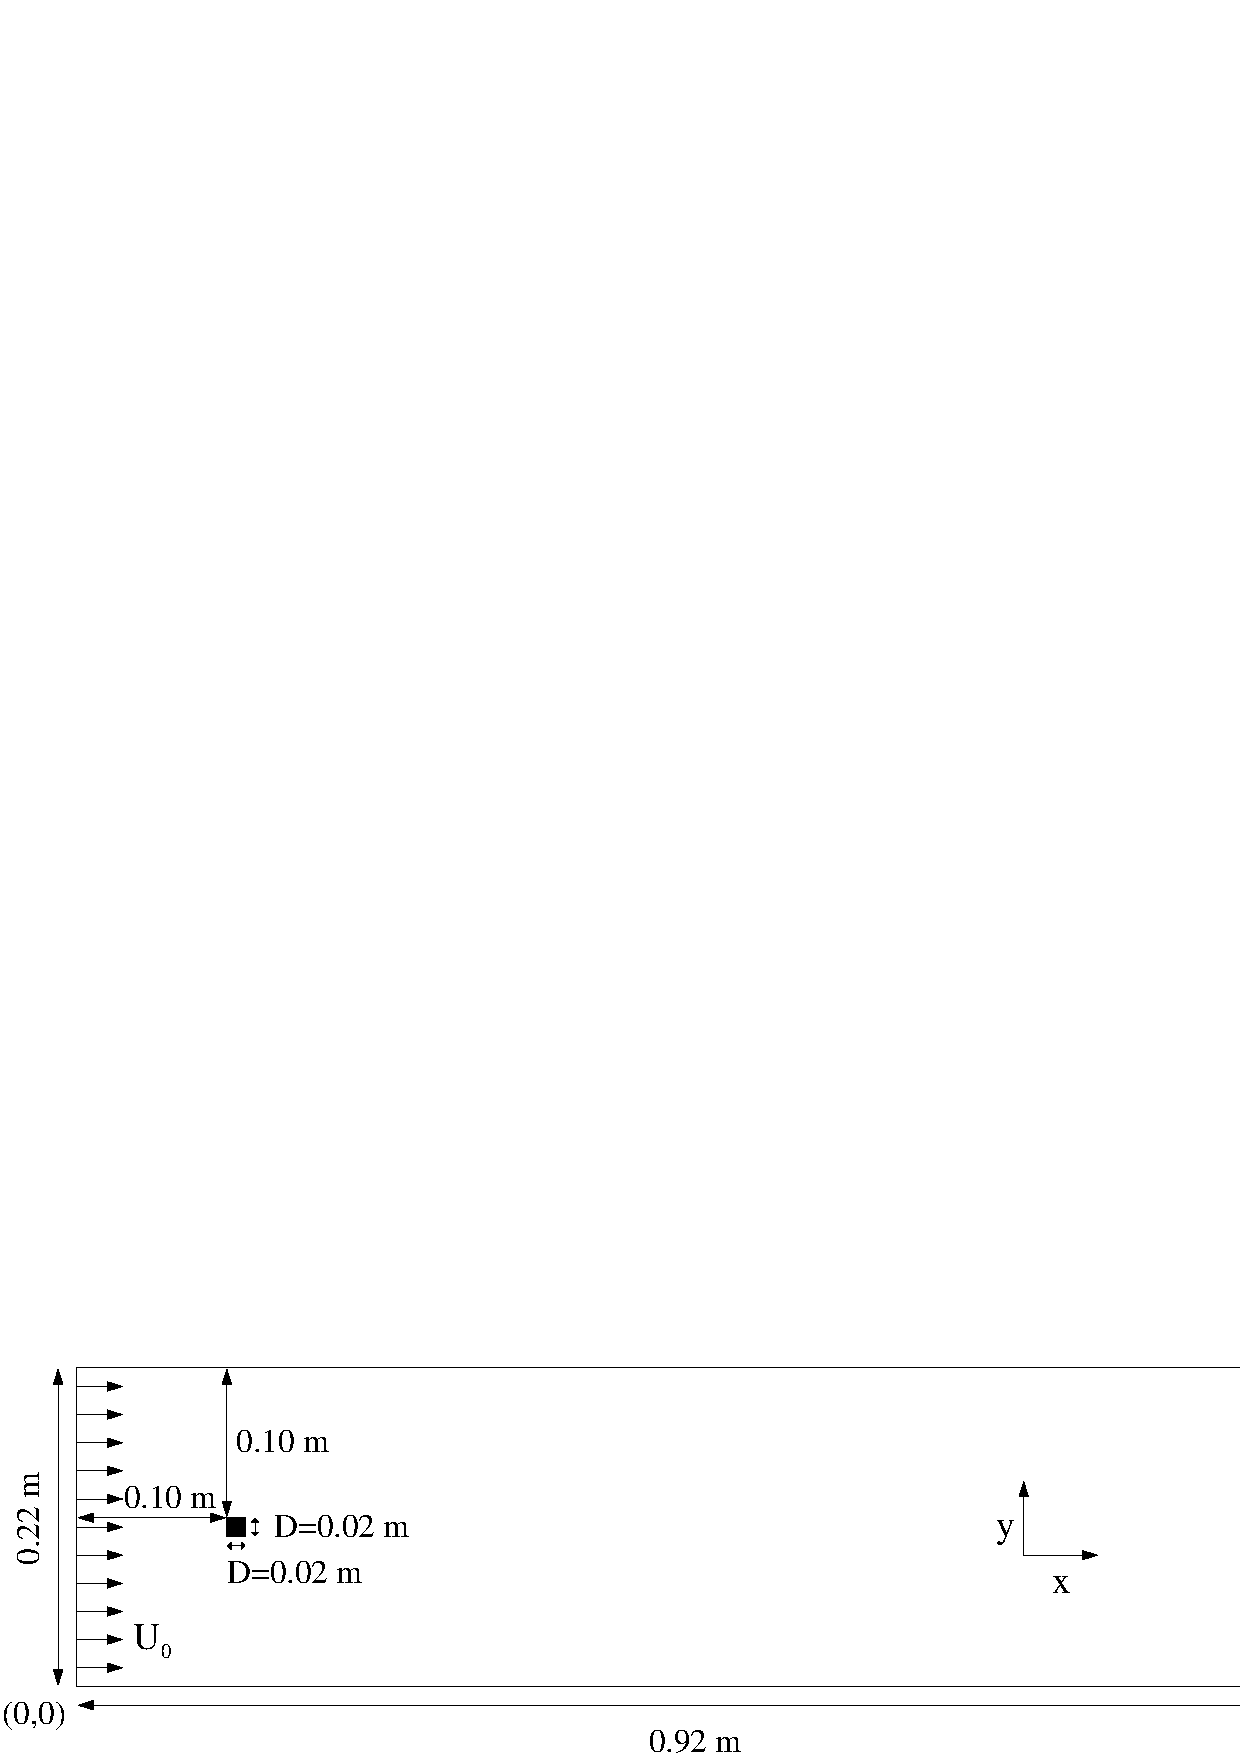
\includegraphics[width=1\textwidth]{PICTURES/Obstacle.pdf}
%\caption{Obstacle}
\end{figure}

\begin{itemize}
\item Fluid: $\mu=3.7 \, 10^{-5} kg.m^{-1}.s^{-1}$, $\rho=2 kg.m^{-3}$ and $R_e=\frac{U_0 H_{inlet} \rho}{\mu} = \frac{1 \times 0.22 \times 2}{3.7 \;10^{-5}} = 11 891$
\item Boundary conditions:\\
    \begin{itemize}
    \item [$\circ$] Inlet with fixed velocity: $U_0=1 m.s^{-1}$
    \item [$\circ$] Outlet with a fixed pressure: $P_0=0$
    \item [$\circ$] Square cylinder: Wall
    \item [$\circ$] Upper and Lower walls: Symmetry
    \end{itemize}
\end{itemize}

\end{block}
\end{frame}
%%%%%%%%%%%%%%%%%%%%%%%%%%%%%%%%%%%%%%%%%%%%%%%%%%%%%%%%%%%%%%%%%%%%%%%%
%%%%%%%%%%%%%%%%%%%%%%%%%%%%%%%%%%%%%%%%%%%%%%%%%%%%%%%%%%%%%%%%%%%%%%%%
\begin{frame}
\frametitle{Create a study}
\begin{block}{}

\begin{itemize}
\item First, you must have already done the commands of the first section.
%we are going to configure the Nedit editor to recognize the Trio\_U keywords in a data file. So run nedit, and select Preferences $\rightarrow$ Save Defaults, then re-initialize the Trio\_U environment (source \$TRIO\_U\_ROOT/bin/Init\_Trio\_U), the message "nedit.rc updated" should appear).
\vspace{0.2cm}

\item Open a terminal and run the commands to create a directory for your studies: \\
\textbf{mkdir -p \; $\sim$/test/yourname}\\
\textbf{cd \; $\sim$/test/yourname}
\vspace{0.2cm}

\item \label{method_copy} Copy a test case from the TRUST database to your study with the command:\\
\textbf{trust -copy\index{trust -copy} Obstacle}\\
\textbf{cd Obstacle}
\vspace{0.2cm}

\item Run the test case with the command:\\
\textbf{trust Obstacle}\\
\vspace{0.2cm}

\item Edit there the data file Obstacle.data and change some lines in order to modify the time step to 0.004s:\\
\textbf{nedit Obstacle.data \&}\\
\end{itemize}

\end{block}
\end{frame}
%%%%%%%%%%%%%%%%%%%%%%%%%%%%%%%%%%%%%%%%%%%%%%%%%%%%%%%%%%%%%%%%%%%%%%%%
%%%%%%%%%%%%%%%%%%%%%%%%%%%%%%%%%%%%%%%%%%%%%%%%%%%%%%%%%%%%%%%%%%%%%%%%
\begin{frame}
\frametitle{Probes and parameters}
\begin{block}{}

\begin{itemize}
\item Add to the post processing block of Obstacle.data the following elements :\\

    \begin{itemize}
    \item [$\circ$] A segment of pressure probes between the points (0.01, 0.12) and (0.91, 0.12).
    \vspace{0.1cm}

    \item [$\circ$] A segment of velocity probes between the points (0.92, 0.00) and (0.92, 0.22) to see the velocity profile behind the square cylinder.
    \vspace{0.1cm}

    \item [$\circ$] Add the vorticity to the fields being post processed and change the writing period to 0.5s. To find the keyword for this field, you can open the User's manual with:\\
    \textbf{trust -doc \&\index{trust -doc \&}}
    \vspace{0.1cm}

    \item [$\circ$] Add the keyword "\textbf{format lata\index{format lata}}" inside the block, just before the keyword \textbf{Champs} in order to use the post processing tool VisIt during and/or after the calculation.
    \vspace{0.1cm}

    \item [$\rightarrow$] You have access to useful resources in the \$TRUST\_ROOT/index.html file with your favourite browser (eg: firefox). Take few minutes to find test case examples containing a particular keyword thanks to the \underline{Keywords} link: \\
    \textbf{firefox \$TRUST\_ROOT/index.html} \\
    or \textbf{trust -index}\\
    \end{itemize}
\end{itemize}

\end{block}
\end{frame}
%%%%%%%%%%%%%%%%%%%%%%%%%%%%%%%%%%%%%%%%%%%%%%%%%%%%%%%%%%%%%%%%%%%%%%%%
%%%%%%%%%%%%%%%%%%%%%%%%%%%%%%%%%%%%%%%%%%%%%%%%%%%%%%%%%%%%%%%%%%%%%%%%
\begin{frame}
\frametitle{Visualization during the calculation}
\begin{block}{}

\begin{itemize}

\item Run the calculation with "-monitor" option to access to a visualization menu: \\
\textbf{trust -monitor\index{trust -monitor} Obstacle}
\vspace{0.1cm}

\item Visualize the evolution of the pressure with the plot number 3. Check also the velocity profile behind the square cylinder. Close the plots (for example, -3 to close the plot 3).
\vspace{0.1cm}

\item Check the convergence monitoring: plot 0 in the first menu to open the convergence menu, then open the 4 following plots:
    \begin{itemize}
    \item [$\circ$] Pressure linear system convergence at each time step
    \item [$\circ$] Residual error $\left\Vert Ax-B \right\Vert$ of the pressure linear system at the last time step
    \item [$\circ$] Time step evolution
    \item [$\circ$] Flow rate error evolution
    \end{itemize}
Type "5" to quit this menu and return to the first one.
\vspace{0.1cm}

\item Visualize the equation residuals (plot 2).
\vspace{0.1cm}


\end{itemize}

\end{block}
\end{frame}
%%%%%%%%%%%%%%%%%%%%%%%%%%%%%%%%%%%%%%%%%%%%%%%%%%%%%%%%%%%%%%%%%%%%%%%%
%%%%%%%%%%%%%%%%%%%%%%%%%%%%%%%%%%%%%%%%%%%%%%%%%%%%%%%%%%%%%%%%%%%%%%%%
\begin{frame}
\frametitle{VisIt}
\begin{block}{}

\begin{itemize}
\item Open the menu "Surface fluxes characteristics" (plot1), visualize:
    \begin{itemize}
    \item [$\circ$] the drag exerted by the fluid on the square Cylinder (plot 1, then 4 for the square), close this menu with 7.
    \item [$\circ$] the "Pressure drag + Friction drag" with 5 and select the Square boundary (4). Each drag is plotted together with the total drag also called viscous drag.
    \end{itemize}
To quit this tool, close the plots and type "\#".

\item Once the calculation is finished, visualize the results with the graphical tool VisIt: \textbf{visit \&}

    \begin{itemize}
    \item [$\circ$] First, we are going to configure VisIt: {\footnotesize{In the menu File $\rightarrow$ Open file, select Off instead of Smart for File grouping option. For the Filter, specify *.lata to list only the LATA results file. Then save your choices, in the menu Options $\rightarrow$ Save Settings.}}

    \item [$\circ$] In the menu File $\rightarrow$ Open file, select the Obstacle.lata file.

    \item [$\circ$] Visualize the mesh in the "Plots" area with "Add $\rightarrow$ Mesh $\rightarrow$ dom" then click on the button "Draw". Zoom and move the mesh in the right window. You will de-zoom with right button (View $\rightarrow$ Reset view) or with a combination of CTRL keypad and left button.

    \item [$\circ$] Visualize the pressure field ({\footnotesize{Plots area: "Add $\rightarrow$ Pseudocolor $\rightarrow$ PRESSION\_SOM\_dom" + Draw then select the last time on the Time slider}})
    \end{itemize}
\end{itemize}

\end{block}
\end{frame}
%%%%%%%%%%%%%%%%%%%%%%%%%%%%%%%%%%%%%%%%%%%%%%%%%%%%%%%%%%%%%%%%%%%%%%%%
%%%%%%%%%%%%%%%%%%%%%%%%%%%%%%%%%%%%%%%%%%%%%%%%%%%%%%%%%%%%%%%%%%%%%%%%
\begin{frame}
\frametitle{VisIt}
\begin{block}{}

\hspace{1cm} $\color{darkblue}\circ$ {\small{Suppress or hide the mesh (Select Mesh then clcik on Delete or Hide/Show).}}\\
\hspace{1cm} $\color{darkblue}\circ$ {\small{Visualize the velocity field ({\footnotesize{Plots area: "Add $\rightarrow$ Vector $\rightarrow$ VITESSE\_SOM\_dom"}}\\
\hspace{1.3cm} {\footnotesize{ + Draw)}}. You can change each plot attributes:}}\\
\vspace{0.05cm}
\hspace{1.5cm} $\color{darkblue}\diamond$ {\footnotesize{click once onto the small arrow "$\blacktriangleright$" then }}\\
\hspace{1.5cm} $\color{darkblue}\diamond$ {\footnotesize{double click on the item Vector (cf the figure below). For example, change \\
\hspace{1.8cm} the amount of vectors plotted (by default 400, increase this number to 40000 \\
\hspace{1.8cm} then click the button "Make default" and save definitively this change with \\
\hspace{1.8cm} the menu Options $\rightarrow$ Save Settings). You need to click Apply to update. Then \\
\hspace{1.8cm} click "Dismiss" to close the window.}}\\

\begin{figure}
\includegraphics[width=0.45\textwidth]{PICTURES/visit3.jpg}
%\caption{Obstacle}
\end{figure}

\hspace{1cm} $\color{darkblue}\circ$ {\small{Print your visualization (File $\rightarrow$ Save window): a PNG file is created into your \\
\hspace{1.3cm} study directory.}}

\end{block}
\end{frame}
%%%%%%%%%%%%%%%%%%%%%%%%%%%%%%%%%%%%%%%%%%%%%%%%%%%%%%%%%%%%%%%%%%%%%%%%
%%%%%%%%%%%%%%%%%%%%%%%%%%%%%%%%%%%%%%%%%%%%%%%%%%%%%%%%%%%%%%%%%%%%%%%%
\begin{frame}
\frametitle{VisIt}
\begin{block}{}

\hspace{1cm} $\color{darkblue}\circ$ {\small{Add a second screen with "Windows $\rightarrow$ Layouts $\rightarrow$ 1x2",}}\\

\hspace{1cm} $\color{darkblue}\circ$ {\small{Plot a pressure horizontal profile:\\}}
\hspace{1.5cm} $\color{darkblue}\diamond$ {\footnotesize{ select the pressure field and thanks to the right button,}} \\ 
\hspace{1.5cm} $\color{darkblue}\diamond$ {\footnotesize{ select "Mode $\rightarrow$ Line out", and define your profile with left button,}} \\
\hspace{1.5cm} $\color{darkblue}\diamond$ {\footnotesize{ click on the origin point, let the left button pushed, and release at the end point.}}\\
\hspace{1.5cm} $\color{darkblue}\diamond$ {\footnotesize{ The profile is shown on the second window.}}\\

\hspace{1cm} $\color{darkblue}\circ$ {\small{You notice that it is necessary to update (button Draw) the right window after \\
\hspace{1.3cm} adding a new plot or changing an option. It is possible to automatically \\
\hspace{1.3cm} update by activating "Auto apply" on the top right of the VisIt's GUI.}}\\

\hspace{1cm} $\color{darkblue}\circ$ {\small{You can create create new fields (expression) with "Controls $\rightarrow$ Expressions \\
\hspace{1.3cm} $\rightarrow$ New" by using existing variables and complex functions and visualize it.}}\\

\hspace{1cm} $\color{darkblue}\circ$ {\small{You can animate your visualization and/or create a movie (File $\rightarrow$ Save movie)}}\\

\hspace{1cm} $\color{darkblue}\circ$ {\small{You can operate calculations on variables with complex queries \\
\hspace{1.3cm} (Controls $\rightarrow$ Query),}}\\

\hspace{1cm} $\color{darkblue}\circ$ {\small{You can save a complex session (File $\rightarrow$ Save session) and reopen it during a \\
\hspace{1.3cm} next analyze with VisIt (File $\rightarrow$ Restore session),}}



\end{block}
\end{frame}
%%%%%%%%%%%%%%%%%%%%%%%%%%%%%%%%%%%%%%%%%%%%%%%%%%%%%%%%%%%%%%%%%%%%%%%%
%%%%%%%%%%%%%%%%%%%%%%%%%%%%%%%%%%%%%%%%%%%%%%%%%%%%%%%%%%%%%%%%%%%%%%%%
\begin{frame}
\frametitle{Outputs and "reprise"}
\begin{block}{}

\hspace{1cm} $\color{darkblue}\circ$ {\small{During a 3D visualization, you will use one of the available Operators \\
\hspace{1.3cm} (In Plots, "Operators $\rightarrow$ Slicing $\rightarrow$ Slice") to create a 2D slice either in a 3D \\
\hspace{1.3cm} space, or projected to a 2D space.}}

\begin{itemize}
\item Edit the different output (*.out) files to read the complete balances (mass, stress, energy, ...) on the whole domain or at the boundaries.
\vspace{0.3cm}
\item  Change the data file to restart the calculation. You will modify \textbf{tinit} (pick in the .err file the last backup time of the previous calculation) and \textbf{tmax} values, and add in the problem definition just before the last "\}":\\
\textbf{reprise binaire Obstacle\_pb.sauv}\\
(The file "Obstacle\_pb.sauv" must have been created during the first run.)
\vspace{0.3cm}
\item Restart the calculation again with:\\
\textbf{trust -monitor\index{trust -monitor} Obstacle}\\
to see that values are added to the first probes during the new calculation.
\end{itemize}

\end{block}
\end{frame}
%%%%%%%%%%%%%%%%%%%%%%%%%%%%%%%%%%%%%%%%%%%%%%%%%%%%%%%%%%%%%%%%%%%%%%%%



\subsection{Obstacle: Parallel calculation}
%%%%%%%%%%%%%%%%%%%%%%%%%%%%%%%%%%%%%%%%%%%%%%%%%%%%%%%%%%%%%%%%%%%%%%%%
\begin{frame}
\begin{columns}[c] 
\column{.45\textwidth}
\tableofcontents[sections={1-6},currentsection, currentsubsection]
\column{.5\textwidth} 
\tableofcontents[sections={7-12},currentsection, currentsubsection]
\end{columns}
\end{frame}
%%%%%%%%%%%%%%%%%%%%%%%%%%%%%%%%%%%%%%%%%%%%%%%%%%%%%%%%%%%%%%%%%%%%%%%%
%%%%%%%%%%%%%%%%%%%%%%%%%%%%%%%%%%%%%%%%%%%%%%%%%%%%%%%%%%%%%%%%%%%%%%%%
\begin{frame}
\frametitle{Parallel calculation: method 1}
\begin{block}{}

The goal of this exercise is to introduce parallelism in the data file of the previous exercise.

\begin{itemize}
\item Go to the previous study (should be done) and after you had suppressed the \textbf{reprise} keyword and set \textbf{tinit} to 0 again in the \textit{Obstacle.data} file, create the two new files:\\
\textbf{cd $\sim$/test/yourname/Obstacle} \\
\textbf{mkdir PARA1} \\
\textbf{cd PARA1} \\
\textbf{cp ../Obstacle.data DEC\_Obstacle.data} \\
\textbf{cp ../Obstacle.data PAR\_Obstacle.data} \\
\textbf{cp ../Obstacle.geo .}\\
\vspace{0.3cm}
\item Edit the first file (\textit{DEC\_Obstacle.data}) to create the partition of the mesh.
\end{itemize}

\end{block}
\end{frame}
%%%%%%%%%%%%%%%%%%%%%%%%%%%%%%%%%%%%%%%%%%%%%%%%%%%%%%%%%%%%%%%%%%%%%%%%
%%%%%%%%%%%%%%%%%%%%%%%%%%%%%%%%%%%%%%%%%%%%%%%%%%%%%%%%%%%%%%%%%%%%%%%%
\begin{frame}
\frametitle{Parallel calculation: method 1}
\begin{block}{}

\begin{itemize}
\item In this file, uncomment the block around the \textbf{Partition} keyword.
    \begin{itemize}
    \item [$\circ$] Here, the partitioning tool \textbf{Tranche} is used. We cut in 2 bands according to X axis and 1 band according to Y axis. 
    \item [$\circ$] The overlapping width \textbf{Larg\_joint} between two parts of the partition should be defined according to the numerical scheme higher order, generally the convective scheme. Its value is generally 1 for the two order scheme, and 2 for the three or four-order scheme like Quick scheme.
    \item [$\circ$] In VEF, you should use \textbf{2} for \textbf{Larg\_joint} except when partitioning a domain where only the conduction equation will be solved.
    \item [$\circ$] At least, the keyword \textbf{Nom\_Zones} is useful to define the name of the files containing the partitioned mesh and to write these files.
    \item [$\circ$] Notice the presence of the keyword \textbf{End} in the "Partition" block: the code will stop to read the dta file at this point!
    \end{itemize}

\item Run the data file: \textbf{trust DEC\_Obstacle}

\item Check the partitioned mesh files DOM\_0000.Zones and DOM\_0001.Zones are generated in your directory: \textbf{ls *.Zones}
\end{itemize}

\end{block}
\end{frame}
%%%%%%%%%%%%%%%%%%%%%%%%%%%%%%%%%%%%%%%%%%%%%%%%%%%%%%%%%%%%%%%%%%%%%%%%
%%%%%%%%%%%%%%%%%%%%%%%%%%%%%%%%%%%%%%%%%%%%%%%%%%%%%%%%%%%%%%%%%%%%%%%%
\begin{frame}
\frametitle{Parallel calculation: method 1}
\begin{block}{}

\begin{itemize}
\item Now, edit the file PAR\_Obstacle.data and comment the read of the mesh
(\textbf{Read\_file}) and uncomment the \textbf{Scatter} keyword which will read the partitioned
mesh. Visualize it with VisIt:\\
\textbf{trust -mesh PAR\_Obstacle}

\item Now, run a parallel calculation with TRUST:\\
\textbf{trust PAR\_Obstacle 2}

\item The post-processing task is identical in sequential or parallel mode. You have the
probes into the .son files and the whole fields in the .lata files. To run VisIt with the
command line:\\
\textbf{visit -o PAR\_Obstacle.lata \&}

\item Select the last time step and visualize the blocks (with Plots: Add $\rightarrow$ Subset $\rightarrow$ blocks)
which represent the parts of the domain partition, then the velocity fields. You can
also visualize a field only on a selected part (block) with the menu Control $\rightarrow$ Subset.

\item To visualize probes after the end of the calculation, you can run the command line:\\
\textbf{trust -probes PAR\_Obstacle}
\end{itemize}

\end{block}
\end{frame}
%%%%%%%%%%%%%%%%%%%%%%%%%%%%%%%%%%%%%%%%%%%%%%%%%%%%%%%%%%%%%%%%%%%%%%%%
%%%%%%%%%%%%%%%%%%%%%%%%%%%%%%%%%%%%%%%%%%%%%%%%%%%%%%%%%%%%%%%%%%%%%%%%
\begin{frame}
\frametitle{Parallel calculation: method 2}
\begin{block}{}

\begin{itemize}
\item The existing tool \textbf{make\_PAR.data} is useful on the data files \underline{which have} the marks MAILLAGE/MESH, DECOUPAGE/PARTITION and LECTURE/SCATTER. If you run the following commands: \\
\textbf{cd $\sim$/test/yourname/Obstacle} \\
\textbf{mkdir PARA2} \\
\textbf{cd PARA2} \\
\textbf{cp ../Obstacle.data exemple.data}\\
\textbf{cp ../Obstacle.geo .}\\
\textbf{make\_PAR.data exemple 3}\\
\textbf{ls *.data *.Zones}\\

\item It will create a DEC\_exemple.data file and will immediately run this file to create a partition with 3 sub zones. The command make\_PAR.data will also create PAR\_exemple.data file and then you will run the calculation by the usual command:\\
\textbf{trust PAR\_exemple 3}
\end{itemize}

\end{block}
\end{frame}
%%%%%%%%%%%%%%%%%%%%%%%%%%%%%%%%%%%%%%%%%%%%%%%%%%%%%%%%%%%%%%%%%%%%%%%%



\subsection{Obstacle: Parallel calculation on a cluster}
%%%%%%%%%%%%%%%%%%%%%%%%%%%%%%%%%%%%%%%%%%%%%%%%%%%%%%%%%%%%%%%%%%%%%%%%
\begin{frame}
\begin{columns}[c] 
\column{.45\textwidth}
\tableofcontents[sections={1-6},currentsection, currentsubsection]
\column{.5\textwidth} 
\tableofcontents[sections={7-12},currentsection, currentsubsection]
\end{columns}
\end{frame}
%%%%%%%%%%%%%%%%%%%%%%%%%%%%%%%%%%%%%%%%%%%%%%%%%%%%%%%%%%%%%%%%%%%%%%%%
%%%%%%%%%%%%%%%%%%%%%%%%%%%%%%%%%%%%%%%%%%%%%%%%%%%%%%%%%%%%%%%%%%%%%%%%
\begin{frame}
\frametitle{Parallel calculation on a cluster}
\begin{block}{}

\begin{itemize}
\item Log onto the cluster callisto and initialize the TRUT version: \\
\vspace{0.2cm}
{\small{
\textbf{ssh -X login@callisto-login1(.intra.cea.fr)} \\
\textbf{source /panfs/ixion/home/triou/TRUST-1.7.1/TRUST/env/env\_TRUST.sh}\\
or 
\textbf{source /home/triou/env\_TRUST\_1.7.1\_patch.sh}\\
}}
\vspace{0.2cm}

\item Copy the study Obstacle:\\
\vspace{0.2cm}
\textbf{cd /panfs/ixion/home/login}\\
\textbf{mkdir -p test/yourname} \\
\textbf{cd test/yourname} \\
\textbf{trust -copy\index{trust -copy} Obstacle} \\
\textbf{cd Obstacle} \\
\vspace{0.2cm}

\item Open Obstacle.data and add \textbf{"format lata\index{format lata}"} in the post-traitement block.
\vspace{0.2cm}

\item Create automatically a 2 partitioned mesh and a parallel datafile with:
\vspace{0.2cm}
\textbf{make\_PAR.data Obstacle}
\end{itemize}

\end{block}
\end{frame}
%%%%%%%%%%%%%%%%%%%%%%%%%%%%%%%%%%%%%%%%%%%%%%%%%%%%%%%%%%%%%%%%%%%%%%%%
%%%%%%%%%%%%%%%%%%%%%%%%%%%%%%%%%%%%%%%%%%%%%%%%%%%%%%%%%%%%%%%%%%%%%%%%
\begin{frame}
\frametitle{Parallel calculation on a cluster}
\begin{block}{}

\begin{itemize}
\item Submit the parallel calculation on 2 cores:\\
\vspace{0.2cm}
\textbf{trust PAR\_Obstacle 2}
\vspace{0.2cm}

\item For clusters, you have to create a submission file:\\
\vspace{0.2cm}
\textbf{trust -create\_sub\_file PAR\_Obstacle 2}
\vspace{0.2cm}

\item Open the file sub\_file and change the name of the job. Note that we will see only the first eight characters of the name of the job in the list of submitted jobs.
\vspace{0.2cm}

\item Submit the job with: \textbf{sbatch sub\_file}
\vspace{0.2cm}

\item Check the state of the job with: \textbf{"squeue"} or \textbf{"squeue $|$ grep login"}
\vspace{0.2cm}

\item You could run VisIt from the cluster but it is not recommanded. But you can run VisIt on your PC and access/visualize the result file on callisto cluster, with File $\rightarrow$ Open File and select callisto in the localhost menu.
\end{itemize}

\end{block}
\end{frame}
%%%%%%%%%%%%%%%%%%%%%%%%%%%%%%%%%%%%%%%%%%%%%%%%%%%%%%%%%%%%%%%%%%%%%%%%



\section{Heat exchange VDF/VEF}
%%%%%%%%%%%%%%%%%%%%%%%%%%%%%%%%%%%%%%%%%%%%%%%%%%%%%%%%%%%%%%%%%%%%%%%%
\begin{frame}
\begin{columns}[c] 
\column{.45\textwidth}
\tableofcontents[sections={1-6},currentsection, currentsubsection]
\column{.5\textwidth} 
\tableofcontents[sections={7-12},currentsection, currentsubsection]
\end{columns}
\end{frame}
%%%%%%%%%%%%%%%%%%%%%%%%%%%%%%%%%%%%%%%%%%%%%%%%%%%%%%%%%%%%%%%%%%%%%%%%
%%%%%%%%%%%%%%%%%%%%%%%%%%%%%%%%%%%%%%%%%%%%%%%%%%%%%%%%%%%%%%%%%%%%%%%%
\begin{frame}
\frametitle{Heat exchange VDF/VEF exercise}
\begin{block}{}


\begin{columns}[c] 
\column{.55\textwidth}
%\begin{figure}
\begin{center}
\includegraphics[width=1.\textwidth]{PICTURES/heat_exchange.pdf}
\end{center}
%\caption{Obstacle}
%\end{figure}

\column{.4\textwidth} 
$$
\begin{array}{ll}
\mbox{\textbf{Fluid:}}      & Pr=\frac{\mu C_p}{\lambda}=1, \\
%                            & Ra=20000,\\
                            & T_{ref}=30^o C,\\
                            & \mu=2 \; 10^{-3} kg.m^{-1}.s^{-1},\\
                            & \rho=2 \; kg.m^{-3},\\
                            & \lambda=1. W.m^{-1}.K^{-1} \\
                            & Cp=500 J.kg^{-1}.K^{-1},\\
                            & \beta=1.10^{-4} K^{-1} \\
                            &  \\
\mbox{\textbf{Solid:}}      & \rho=1000 kg.m^{-3} \\
                            & \lambda=250 W.m^{-1}.K^{-1} \\
                            & Cp=100 J.kg^{-1}.K^{-1}
\end{array}
$$

\end{columns}

\end{block}
\end{frame}
%%%%%%%%%%%%%%%%%%%%%%%%%%%%%%%%%%%%%%%%%%%%%%%%%%%%%%%%%%%%%%%%%%%%%%%%
%%%%%%%%%%%%%%%%%%%%%%%%%%%%%%%%%%%%%%%%%%%%%%%%%%%%%%%%%%%%%%%%%%%%%%%%
\begin{frame}
\frametitle{Heat exchange VDF/VEF exercise}
\begin{block}{}

\begin{itemize}
\item Create a new study Coupling\_VDF by copying the docond study:\\
\textbf{cd $\sim$/test/yourname} \\
\textbf{trust -copy\index{trust -copy} docond} \\
\textbf{mv docond Coupling\_VDF} \\
\textbf{cd Coupling\_VDF} \\

\item Check the fluid and solid characteristics inside the docond.data file.

\item This coupled problem is constitued by 2 domains of calculation with a mesh of 10x10 cells ($\Delta x = \Delta y = 0.1m$) created with 3 blocks. 

\item Modify the data file to have the 2 domains on a mesh of 40x40 cells ($\Delta x= \Delta y=0.025m$). For this, you will change the number of nodes for each block like this:\\
First block (Cavite1): 4 11 $\rightarrow$ 13 41 \\
Second block (Cavite2): 8 4 $\rightarrow$ 29 13 \\ 
Third block (Cavite3): 8 8  $\rightarrow$ 29 29 \\

\item Change \textbf{"format lml\index{format lml}"} to \textbf{"format lata"} into the two problems definition and run the calculation and check the evolution. 
\end{itemize}

\end{block}
\end{frame}
%%%%%%%%%%%%%%%%%%%%%%%%%%%%%%%%%%%%%%%%%%%%%%%%%%%%%%%%%%%%%%%%%%%%%%%%
%%%%%%%%%%%%%%%%%%%%%%%%%%%%%%%%%%%%%%%%%%%%%%%%%%%%%%%%%%%%%%%%%%%%%%%%
\begin{frame}
\frametitle{Heat exchange VDF/VEF exercise}
\begin{block}{}

\begin{itemize}
\item Then post process the temperature field with the tool VisIt. A natural convection cell appears. Change the colour tables for the temperature to have the same one on the 2 domains.

\item We are going to change the discretization of the test case. Triangulate the domains with the keyword \textbf{Trianguler\_H} (See the syntax in the User's manual). Give an unstructured aspect to the 2 meshes thanks to the following keyword : \\
\textbf{Transformer name\_of\_domain \; x*(1-0.5*y*y) \; y*(1+0.1*x*y)}

\item Substitute the discretization VDF (pressure nodes at the element center) to VEFPreP1B (pressure nodes at the element center and nodes).

\item Check the meshes with: \\
\textbf{trust -mesh docond}

\item Run the calculation with:\\
\textbf{trust -monitor\index{trust -monitor} docond}

\item Follow the residuals (plot number 2) and a probe evolution (for example temperature), to see when convergence is reached.
\end{itemize}

\end{block}
\end{frame}
%%%%%%%%%%%%%%%%%%%%%%%%%%%%%%%%%%%%%%%%%%%%%%%%%%%%%%%%%%%%%%%%%%%%%%%%
%%%%%%%%%%%%%%%%%%%%%%%%%%%%%%%%%%%%%%%%%%%%%%%%%%%%%%%%%%%%%%%%%%%%%%%%
\begin{frame}
\frametitle{Heat exchange VDF/VEF exercise}
\begin{block}{}

\begin{itemize}
\item Post-process the results and compare with VDF discretization about the CPU performance: the VEF calculation is running 10 times slower (cause higher number of pressure unknowns and smaller time steps). Study the docond.out file to see the time steps for each equation.

\item Accelerate the calculation by impliciting the diffusion operators of each equation with \textbf{diffusion\_implicite} option in the explicit Euler scheme (check again the User's manual: \textbf{trust -doc \&\index{trust -doc \&}}). Run the calculation.

\item \label{schema_impl} Use a full implicit scheme now (suppress \textbf{diffusion\_implicite}), by substituting \textbf{Schema\_Euler\_Explicite} by \textbf{Schema\_Euler\_implicite} and adding the \textbf{Implicite} solver. Have a look at the User's manual for the \textbf{gmres} options and define accordingly to the advices given into the User's manual, a value for \textbf{facsec, facsec\_max}. You block will looks like:\\
\textbf{Solveur Implicite \{ solveur gmres \{ diag seuil 1e-30 nb\_it\_max 5 impr \}  seuil\_convergence\_implicite 0.01  \} }

\item Run the calculation.
\end{itemize}

\end{block}
\end{frame}
%%%%%%%%%%%%%%%%%%%%%%%%%%%%%%%%%%%%%%%%%%%%%%%%%%%%%%%%%%%%%%%%%%%%%%%%



\section{Low mach number flow}
%%%%%%%%%%%%%%%%%%%%%%%%%%%%%%%%%%%%%%%%%%%%%%%%%%%%%%%%%%%%%%%%%%%%%%%%
\begin{frame}
\begin{columns}[c] 
\column{.45\textwidth}
\tableofcontents[sections={1-6},currentsection, currentsubsection]
\column{.5\textwidth} 
\tableofcontents[sections={7-12},currentsection, currentsubsection]
\end{columns}
\end{frame}
%%%%%%%%%%%%%%%%%%%%%%%%%%%%%%%%%%%%%%%%%%%%%%%%%%%%%%%%%%%%%%%%%%%%%%%%
%%%%%%%%%%%%%%%%%%%%%%%%%%%%%%%%%%%%%%%%%%%%%%%%%%%%%%%%%%%%%%%%%%%%%%%%
\begin{frame}
\frametitle{Low mach number flow}
\begin{block}{}

\begin{itemize}
\item Open a terminal and create a directory using Unix commands, and copy the study \textbf{TP\_Temp\_QC\_VEF} (it is a 2D simulation of helium gas flow from left to right between two heated walls):\\
\textbf{mkdir -p $\sim$/test/yourname}\\
\textbf{trust -copy\index{trust -copy} TP\_Temp\_QC\_VEF}\\
\textbf{cd TP\_Temp\_QC\_VEF}

\item Open the TRUST User's manual with (it will be useful to search for keywords in this exercice): \textbf{trust -doc \&\index{trust -doc \&}}

\item Edit the data file with your favourite editor (\textbf{nedit} is recommended because it is configured to recognize TRUST syntax):\\
\textbf{nedit TP\_Temp\_QC\_VEF.data \&}

\item Modify the data file in order to:
    \begin{itemize}
    \item [$\circ$] Change the geometry and the mesh:
    \begin{figure}
    \includegraphics[width=0.5\textwidth]{PICTURES/low_mach.pdf}
    %\caption{Obstacle}
    \end{figure}
    \end{itemize}
\end{itemize}

\end{block}
\end{frame}
%%%%%%%%%%%%%%%%%%%%%%%%%%%%%%%%%%%%%%%%%%%%%%%%%%%%%%%%%%%%%%%%%%%%%%%%
%%%%%%%%%%%%%%%%%%%%%%%%%%%%%%%%%%%%%%%%%%%%%%%%%%%%%%%%%%%%%%%%%%%%%%%%
\begin{frame}
\frametitle{Low mach number flow}
\begin{block}{}

\hspace{1cm} $\color{darkblue}\circ$ {\small{Add several probes (velocity, volume mass, temperature) near the upper right\\
\hspace{1.3cm} corner of the geometry at location (x,y)=(4,1).}} \\

\hspace{1cm} $\color{darkblue}\circ$ {\small{Add a probe \textbf{"segment"} (with 9 points) between the locations (x,y)=(4,0.05) \\
\hspace{1.3cm} and (x,y)=(4,0.95) for the temperature field.}}

\hspace{1cm} $\color{darkblue}\circ$ {\small{Write the results with the \textbf{LATA} format and change the \textbf{dt\_post} period to 1s. }}\\

\hspace{1cm} $\color{darkblue}\circ$ {\small{We are looking for the stationary state, so suppress tmax keyword and change \\
\hspace{1.3cm} the \textbf{seuil\_statio} $\varepsilon$ value to 10 ($|dT/dt|<\varepsilon$ and $dt \sim 0.001s$ so $|dT|<0.01$).}}\\

\hspace{1cm} $\color{darkblue}\circ$ {\small{Add the keyword \textbf{impr} into the pressure solver to print its convergence.}}

\begin{itemize}
\item Run the simulation with the TRUST command:\\
\textbf{trust -monitor\index{trust -monitor} TP\_Temp\_QC\_VEF}\\
    \begin{itemize}
    \item [$\circ$]Check the convergence information by entering 0 (convergence monitoring in the menu). Visualize the 3 plots:
        \begin{itemize}
        \item [$\diamond$] Conjugate Gradient iterations number at each time step,
        \item [$\diamond$] Error evolution of Conjugate Gradient resolution at each time step,
        \item [$\diamond$] Time step evolution.
        \end{itemize}
    \end{itemize}
\end{itemize}

\end{block}
\end{frame}
%%%%%%%%%%%%%%%%%%%%%%%%%%%%%%%%%%%%%%%%%%%%%%%%%%%%%%%%%%%%%%%%%%%%%%%%
%%%%%%%%%%%%%%%%%%%%%%%%%%%%%%%%%%%%%%%%%%%%%%%%%%%%%%%%%%%%%%%%%%%%%%%%
\begin{frame}
\frametitle{Low mach number flow}
\begin{block}{}

\hspace{1cm} $\color{darkblue}\circ$ {\small{And check mass flow rate (absolute and relative values) in the\\
\hspace{1.3cm} TP\_Temp\_QC\_VEF.out file: \\
\hspace{1.3cm} \textbf{nedit TP\_Temp\_QC\_VEF.out \&} }}\\

\hspace{1cm} $\color{darkblue}\circ$ {\small{Once the calculation finishes, visualize the results by running \textbf{VisIt}:\\
\hspace{1.3cm} \textbf{visit -o TP\_Temp\_QC\_VEF.lata \&} }}\\

\hspace{1cm} $\color{darkblue}\circ$ {\small{See the mesh (Plots: "Add $\rightarrow$ Mesh $\rightarrow$ dom $\rightarrow$ Draw").}}

\hspace{1cm} $\color{darkblue}\circ$ {\small{Visualize the temperature field (Select the last Time with the slicer, then  \\
\hspace{1.3cm} Plots: "Add $\rightarrow$ Pseudo Color $\rightarrow$ TEMPERATURE\_SOM\_dom  $\rightarrow$ Draw")}}

\hspace{1cm} $\color{darkblue}\circ$ {\small{Suppress or hide the mesh (Select "Mesh-dom" in the list of plots then \\
\hspace{1.3cm} "Delete" or "Hide/Show")}}

\hspace{1cm} $\color{darkblue}\circ$ {\small{Visualize the velocity field (Add $\rightarrow$ Vector $\rightarrow$ VITESSE\_SOM\_dom $\rightarrow$ Draw).}}

\hspace{1cm} $\color{darkblue}\circ$ {\small{Select the Zoom mode with the right button of the mouse (Mode $\rightarrow$ Zoom) \\
\hspace{1.3cm} then zoom by selecting an area in the plot. To de-zoom push "Ctrl" button \\
\hspace{1.3cm} and select an area with the left button or with the right button select \\
\hspace{1.3cm} "View $\rightarrow$ Reset view".}}

\hspace{1cm} $\color{darkblue}\circ$ {\small{Print your visualization (File $\rightarrow$ Set Save options $\rightarrow$ File type $\rightarrow$ Select a type \\
\hspace{1.3cm}  $\rightarrow$ Save): a file named visit*** is created into your study directory.}}

\end{block}
\end{frame}
%%%%%%%%%%%%%%%%%%%%%%%%%%%%%%%%%%%%%%%%%%%%%%%%%%%%%%%%%%%%%%%%%%%%%%%%
%%%%%%%%%%%%%%%%%%%%%%%%%%%%%%%%%%%%%%%%%%%%%%%%%%%%%%%%%%%%%%%%%%%%%%%%
\begin{frame}
\frametitle{Low mach number flow}
\begin{block}{}

\hspace{1cm} $\color{darkblue}\circ$ {\small{Add a second screen with "Window $\rightarrow$ Layout $\rightarrow$ 1x2".}}

\hspace{1cm} $\color{darkblue}\circ$ {\small{Plot a temperature horizontal profile (Select the temperature field and \\
\hspace{1.3cm} thanks to the right button, select "Mode $\rightarrow$ Lineout", and define your \\
\hspace{1.3cm} profile with left button): the profile is shown on the second window.}}

\begin{itemize}
\item Substitute the time scheme by an implicit time scheme (like \textbf{schema\_euler\_implicite}). 

\item Use the \textbf{implicite} solver and specify \textbf{facsec} and \textbf{facsec\_max} parameters according to the advices given into the User's manual (search for the \textbf{schema\_euler\_implicite} keyword for the according syntax). You can also see the informations at the end of the Heat exchange VDF/VEF exercise at p.\pageref{schema_impl}.

\item Run the calculation with this time scheme: \\
{\footnotesize{\textbf{trust TP\_Temp\_QC\_VEF.data 1$>$TP\_Temp\_QC\_VEF.out 2$>$TP\_Temp\_QC\_VEF.err}}}

\item Edit the following file where is located information about time-step used dt, stability time-step dt\_stab, \textbf{facsec} evolution (dt=dt\_stab*facsec), residuals for each equation: \\
\textbf{nedit TP\_Temp\_QC\_VEF.dt\_ev \&}
\end{itemize}

\end{block}
\end{frame}
%%%%%%%%%%%%%%%%%%%%%%%%%%%%%%%%%%%%%%%%%%%%%%%%%%%%%%%%%%%%%%%%%%%%%%%%
%%%%%%%%%%%%%%%%%%%%%%%%%%%%%%%%%%%%%%%%%%%%%%%%%%%%%%%%%%%%%%%%%%%%%%%%
\begin{frame}
\frametitle{Low mach number flow}
\begin{block}{}

\begin{itemize}

\item  If everything is OK, try to fine tune the speed convergence of the implicit solver with the value of \textbf{seuil\_convergence\_implicite} keyword (look inside the TP\_Temp\_QC\_VEF.out file and check that the number of iterations for GMRES is between 3 and 5, it is enough to quickly converge).

\item  To restart a calculation, you will need to change the \textbf{tinit} value into the data file (pick up the last save time in the \textbf{.err} file) and insert into the data file in the problem definition the following keywords: \\
\textbf{reprise binaire TP\_Temp\_QC\_VEF\_pb.sauv}

\item  Then run the calculation with: \\
{\footnotesize{\textbf{trust TP\_Temp\_QC\_VEF.data 1$>$TP\_Temp\_QC\_VEF.out 2$>$TP\_Temp\_QC\_VEF.err}}} \\
or \\
\textbf{trust -monitor\index{trust -monitor} TP\_Temp\_QC\_VEF.data} which creates automaticaly the .out and .err files.

\end{itemize}

\end{block}
\end{frame}
%%%%%%%%%%%%%%%%%%%%%%%%%%%%%%%%%%%%%%%%%%%%%%%%%%%%%%%%%%%%%%%%%%%%%%%%



\section{Periodic 3D channel flow}
%%%%%%%%%%%%%%%%%%%%%%%%%%%%%%%%%%%%%%%%%%%%%%%%%%%%%%%%%%%%%%%%%%%%%%%%
\begin{frame}
\begin{columns}[c] 
\column{.45\textwidth}
\tableofcontents[sections={1-6},currentsection, currentsubsection]
\column{.5\textwidth} 
\tableofcontents[sections={7-12},currentsection, currentsubsection]
\end{columns}
\end{frame}
%%%%%%%%%%%%%%%%%%%%%%%%%%%%%%%%%%%%%%%%%%%%%%%%%%%%%%%%%%%%%%%%%%%%%%%%
%%%%%%%%%%%%%%%%%%%%%%%%%%%%%%%%%%%%%%%%%%%%%%%%%%%%%%%%%%%%%%%%%%%%%%%%
\begin{frame}
\frametitle{Periodic 3D channel flow}
\begin{block}{}

\begin{figure}
\includegraphics[width=0.45\textwidth]{PICTURES/periodic3D.png}
%\caption{Obstacle}
\end{figure}

\textbf{Fluid:} $Re=2000$, $\rho=2 kg.m^{-3}$, $\mu=0.01 kg.m^{-1}.s^{-1}$, initial velocity $V0=1m/s$, periodic boundary condition on Z direction.

\begin{itemize}
\item Copy the study named \textbf{P1toP1Bulle} like explained page \pageref{method_copy}. It simulates a 3D incompressible laminar flow ($Re=2000$) with periodic boundary according Z direction only.

\item Open the P1toP1Bulle.data file and use \textbf{RegroupeBord} keyword to merge Entree and Sortie boundaries into a single one named periox. 
\end{itemize}

\end{block}
\end{frame}
%%%%%%%%%%%%%%%%%%%%%%%%%%%%%%%%%%%%%%%%%%%%%%%%%%%%%%%%%%%%%%%%%%%%%%%%
%%%%%%%%%%%%%%%%%%%%%%%%%%%%%%%%%%%%%%%%%%%%%%%%%%%%%%%%%%%%%%%%%%%%%%%%
\begin{frame}
\frametitle{Periodic 3D channel flow}
\begin{block}{}

\begin{itemize}
\item Change the boundary conditions to apply a periodic boundary on the new boundary. 

\item Change the velocity initial condition to $U_0=(1,0,0)$. 

\item Set the option \textbf{diffusion\_implicite} to 1 into the Euler scheme to implicit the diffusive operator of the Navier Stokes equation.

\item You have now a 3D calculation with periodic condition on X and Z directions. Run the calculation on 30 time-steps (keyword \textbf{nb\_pas\_dt\_max}).

\item Have a look at the P1toP1Bulle\_pb\_Debit.out file, check the flow rate on the periox boundary. Why does it decrease?

\item Add the \textbf{Canal\_perio} source term in the Navier Stokes equation of the data file and run again the calculation to check the flow rate evolution on 30 time steps. 

\item Look for the pressure and viscous forces applied to the cylinder inside the .out files.
\end{itemize}

\end{block}
\end{frame}
%%%%%%%%%%%%%%%%%%%%%%%%%%%%%%%%%%%%%%%%%%%%%%%%%%%%%%%%%%%%%%%%%%%%%%%%
%%%%%%%%%%%%%%%%%%%%%%%%%%%%%%%%%%%%%%%%%%%%%%%%%%%%%%%%%%%%%%%%%%%%%%%%
\begin{frame}
\frametitle{Periodic 3D channel flow}
\begin{block}{}

\begin{itemize}
\item Now, the calculation domain is a rotating channel according to Z direction with a constant velocity $\Omega=1 rad/s$. 

\item Add the \textbf{Acceleration} source term in the Navier Stokes equation. Suppress the \textbf{nb\_pas\_dt\_max} keyword and set \textbf{tmax} to 100s.

\item Add, if you wish, velocity or statistic calculation in the post processing instructions. 

\item Run the calculation.

\item You can create a uniformly refined mesh using for instance the keyword \textbf{Raffiner\_Anisotrope}.

\item Then improve the calculation speed on this mesh, you could try to use a coarse discretization \textbf{P1} (\textbf{Read dis \{ P1 \}} keywords) with less pressure unknowns. On this mesh, it runs 3 times faster than P1Bulle but with less accuracy: 8452 unknowns compare to 49221 unknowns.
\end{itemize}

\end{block}
\end{frame}
%%%%%%%%%%%%%%%%%%%%%%%%%%%%%%%%%%%%%%%%%%%%%%%%%%%%%%%%%%%%%%%%%%%%%%%%
%%%%%%%%%%%%%%%%%%%%%%%%%%%%%%%%%%%%%%%%%%%%%%%%%%%%%%%%%%%%%%%%%%%%%%%%
\begin{frame}
\frametitle{Periodic 3D channel flow}
\begin{block}{}

\begin{itemize}
\item Then restart the calculation with \textbf{VEFPreP1B} discretization by reading the velocity field with \textbf{Champ\_fonc\_reprise} keyword in the initial conditions for the velocity:\\
\textbf{vitesse champ\_fonc\_reprise P1toP1Bulle\_pb.xyz  pb  vitesse  last\_time} \\
\underline{This will be useful to reach the quasi-stationary state faster.}

\item You can also use implicit scheme (change the scheme to \textbf{Schema\_Euler\_implicite} scheme and use an \textbf{Implicite} solver) \underline{only if you are looking for the stationary state}.\\ 
You can also see the informations at the end of the Heat exchange VDF/VEF exercise page \pageref{schema_impl}.
\end{itemize}

\end{block}
\end{frame}
%%%%%%%%%%%%%%%%%%%%%%%%%%%%%%%%%%%%%%%%%%%%%%%%%%%%%%%%%%%%%%%%%%%%%%%%


\section{Constituents and turbulent flow}
%%%%%%%%%%%%%%%%%%%%%%%%%%%%%%%%%%%%%%%%%%%%%%%%%%%%%%%%%%%%%%%%%%%%%%%%
\begin{frame}
\begin{columns}[c] 
\column{.45\textwidth}
\tableofcontents[sections={1-6},currentsection, currentsubsection]
\column{.5\textwidth} 
\tableofcontents[sections={7-12},currentsection, currentsubsection]
\end{columns}
\end{frame}
%%%%%%%%%%%%%%%%%%%%%%%%%%%%%%%%%%%%%%%%%%%%%%%%%%%%%%%%%%%%%%%%%%%%%%%%
%%%%%%%%%%%%%%%%%%%%%%%%%%%%%%%%%%%%%%%%%%%%%%%%%%%%%%%%%%%%%%%%%%%%%%%%
\begin{frame}
\frametitle{Constituents and turbulent flow}
\begin{block}{}

\begin{figure}
\includegraphics[width=0.75\textwidth]{PICTURES/marche.pdf}
%\caption{Obstacle}
\end{figure}

\textbf{Fluid:} $\mu=3.7 \, 10^{-5} kg.m^{-1}.s^{-1}, \rho=2 \, kg.m^{-3}, R_e=\frac{U_0 H_{inlet} \rho}{\mu} =54054$

\textbf{Boundary conditions:} \\
Inlet with fixed velocity: $U_0=1 m.s^{-1}$, C1\_eps=$10^{-2}$, C2\_eps=$10^{-3}$ (dimensionless values)\\
Outlet with a fixed pressure: $P_0=0$, C1\_eps=0, C2\_eps=0 \\
Upper and lower walls: No slip wall ($U=0$) and non-porous wall ($\partial C_i/\partial n=0$)

\begin{itemize}
\item Copy the study named \textbf{Marche} like explained page \pageref{method_copy}. It simulates a 2D incompressible turbulent flow with a K-Eps model in the geometry described above.
\end{itemize}

\end{block}
\end{frame}
%%%%%%%%%%%%%%%%%%%%%%%%%%%%%%%%%%%%%%%%%%%%%%%%%%%%%%%%%%%%%%%%%%%%%%%%
%%%%%%%%%%%%%%%%%%%%%%%%%%%%%%%%%%%%%%%%%%%%%%%%%%%%%%%%%%%%%%%%%%%%%%%%
\begin{frame}
\frametitle{Constituents and turbulent flow}
\begin{block}{}

\begin{itemize}
\item Copy also the \textbf{Constituants} study which will give you examples for constituents keyword used for a 2D incompressible laminar flow.

\item Edit your data file in the Marche directory. First, change the name of the problem in order to add concentration equations (look for the good keyword in the User manual).

\item Add 3 constituents with the same diffusivities ($\alpha=1m/s$) and associate the constituents to the problem.

\item Define the concentration equation into the problem (remember that concentrations will be a vector of 3 components) with correct initials ($C_1=0, C_2=0, C_3=0$) and boundaries conditions.

\item Use the Schmidt model to close the turbulence modelization in the  concentration equation.

\item Change the sources of the Navier-Stokes turbulence model to a \textbf{Source\_Transport\_K\_Eps\_aniso\_concen \{ C1\_eps 1.44 C2\_eps 1.92 C3\_eps 1. \} } to fit with the new concentration equation.
\end{itemize}

\end{block}
\end{frame}
%%%%%%%%%%%%%%%%%%%%%%%%%%%%%%%%%%%%%%%%%%%%%%%%%%%%%%%%%%%%%%%%%%%%%%%%
%%%%%%%%%%%%%%%%%%%%%%%%%%%%%%%%%%%%%%%%%%%%%%%%%%%%%%%%%%%%%%%%%%%%%%%%
\begin{frame}
\frametitle{Constituents and turbulent flow}
\begin{block}{}

\begin{itemize}
\item Add into the fluid definition, the volume expansion coefficient for the concentration: \textbf{beta\_co} as an uniform field fixed to 0.

\item You have also to add a gravity field which can be initialized to 0.

\item Run the calculation to see if it is ok.

\item Define a sub domain (in grey on the previous picture) with the keyword \textbf{Sous\_Zone} (like in PCR data file).

\item Add a source term for the second constituent only ($S_2=1m^{-3}$) applied on the sub domain thanks to the keyword \textbf{Champ\_Uniforme\_Morceaux}.

\item Add \textbf{format lata\index{format lata}} in te post-processing block.

\item Add the keyword \textbf{concentration0, concentration1, concentration2} in the \textbf{Champs} of the post-processing block to write the 3 concentrations into the .lata results file.

\item Run the calculation and check the results.
\end{itemize}

\end{block}
\end{frame}
%%%%%%%%%%%%%%%%%%%%%%%%%%%%%%%%%%%%%%%%%%%%%%%%%%%%%%%%%%%%%%%%%%%%%%%%



\section{3D turbulent flow in a curved pipe}
%%%%%%%%%%%%%%%%%%%%%%%%%%%%%%%%%%%%%%%%%%%%%%%%%%%%%%%%%%%%%%%%%%%%%%%%
\begin{frame}
\begin{columns}[c] 
\column{.45\textwidth}
\tableofcontents[sections={1-6},currentsection, currentsubsection]
\column{.5\textwidth} 
\tableofcontents[sections={7-12},currentsection, currentsubsection]
\end{columns}
\end{frame}
%%%%%%%%%%%%%%%%%%%%%%%%%%%%%%%%%%%%%%%%%%%%%%%%%%%%%%%%%%%%%%%%%%%%%%%%
%%%%%%%%%%%%%%%%%%%%%%%%%%%%%%%%%%%%%%%%%%%%%%%%%%%%%%%%%%%%%%%%%%%%%%%%
\begin{frame}
\frametitle{3D turbulent flow in a curved pipe}
\begin{block}{TrioCFD}

\begin{figure}
\includegraphics[width=0.25\textwidth]{PICTURES/pipe2.jpg}
\includegraphics[width=0.25\textwidth]{PICTURES/pipe1.jpg}
%\caption{Obstacle}
\end{figure}

Goals:
\begin{itemize}
\item Use of a RANS or LES model.
\item Use of a periodic box to initialize a fully developed turbulent flow.
\item Use of the TrioCFD parallel capabilities.
\end{itemize}

\end{block}
\end{frame}
%%%%%%%%%%%%%%%%%%%%%%%%%%%%%%%%%%%%%%%%%%%%%%%%%%%%%%%%%%%%%%%%%%%%%%%%
%%%%%%%%%%%%%%%%%%%%%%%%%%%%%%%%%%%%%%%%%%%%%%%%%%%%%%%%%%%%%%%%%%%%%%%%
\begin{frame}
\frametitle{3D turbulent flow in a curved pipe}
\begin{block}{TrioCFD}

\begin{itemize}
\item First initialize TrioCFD environnement :\\
{\small{
\textbf{source /home/triou/env\_TrioCFD\_1.7.1\_patch.sh }\\
\textbf{echo \$exec} \\
\textbf{export TrioCFD\_ROOT=\`\,dirname \$exec \`} \\
\textbf{echo \$TrioCFD\_ROOT} \\
}}

\item Create a new directory and copy some data:\\
{\small{
\textbf{mkdir -p $\sim$/test/yourname/PeriodicBox} \\
\textbf{cd $\sim$/test/yourname/PeriodicBox} \\
\textbf{cp \$TrioCFD\_ROOT/validation/share/Validation/Rapports\_automatiques/} \\
\hspace{4cm} \textbf{Validant/pas\_fini/PeriodicBox/src/* \; .} \\
}}
\vspace{0.2cm}
Notice that this directory correspond to an automated validation test case. 
If you want to run it and generated the pdf report, see the last exercise of this tutorial named "Validation form", but be carefull this case is very slow !
\end{itemize}

\end{block}
\end{frame}
%%%%%%%%%%%%%%%%%%%%%%%%%%%%%%%%%%%%%%%%%%%%%%%%%%%%%%%%%%%%%%%%%%%%%%%%
%%%%%%%%%%%%%%%%%%%%%%%%%%%%%%%%%%%%%%%%%%%%%%%%%%%%%%%%%%%%%%%%%%%%%%%%
\begin{frame}
\frametitle{3D turbulent flow in a curved pipe}
\begin{block}{TrioCFD}

\begin{itemize}
\item There are several files :\\
    \begin{itemize}
    \item [$\circ$] \textit{BuildMeshes.data}: To build the meshes\\
    \item [$\circ$] \textit{PeriodicBoxRANS.data}: To run the flow in the box with RANS model\\
    \item [$\circ$] \textit{DomainFlowRANS.data}: To run the flow in the domain with inlet steady conditions from the box domain\\
    \item [$\circ$] \textit{PeriodicBoxLES.data}: To run the flow in the box with LES model\\
    \item [$\circ$] \textit{DomainFlowLES.data}: To run the flow in the domain with inlet unsteady conditions from the box domain
    \end{itemize}

\item First, edit and read the BuildMeshes.data file.

\item If you wish to run a RANS simulation, open the PeriodicBoxRANS.data and DomainFlowRANS.data files.

\item Or if you wish to run a LES simulation, open the PeriodicBoxLES.data and DomainFlowLES.data files.
\end{itemize}

\end{block}
\end{frame}
%%%%%%%%%%%%%%%%%%%%%%%%%%%%%%%%%%%%%%%%%%%%%%%%%%%%%%%%%%%%%%%%%%%%%%%%
%%%%%%%%%%%%%%%%%%%%%%%%%%%%%%%%%%%%%%%%%%%%%%%%%%%%%%%%%%%%%%%%%%%%%%%%
\begin{frame}
\frametitle{3D turbulent flow in a curved pipe}
\begin{block}{TrioCFD}

\begin{itemize}
\item Then build the meshes:\\
\textbf{./prepare} \\
\textbf{trust BuildMeshes} \\
Notice that we use \textbf{"trust"} command line because this script will use the variable \$exec which is the path to the TrioCFD executable.

\item You can visualize the partitioned meshes with (MODEL=RANS or LES): \\
\textbf{trust -mesh PeriodicBoxMODEL}

\item Then, fix the maximal number of time steps in the time scheme using \textbf{nb\_pas\_dt\_max} to 100 in the files PeriodicBoxRANS and PeriodicBoxLES and run the 2 cores parallel calculations, to initialize the turbulent flow in the box: \\
\textbf{trust PeriodicBoxRANS 2} \\
\textbf{trust PeriodicBoxLES 2} \\
(The full calculation in RANS takes approximatively 1h and 10h in LES.)
\end{itemize}

\end{block}
\end{frame}
%%%%%%%%%%%%%%%%%%%%%%%%%%%%%%%%%%%%%%%%%%%%%%%%%%%%%%%%%%%%%%%%%%%%%%%%
%%%%%%%%%%%%%%%%%%%%%%%%%%%%%%%%%%%%%%%%%%%%%%%%%%%%%%%%%%%%%%%%%%%%%%%%
\begin{frame}
\frametitle{3D turbulent flow in a curved pipe}
\begin{block}{TrioCFD}

\begin{itemize}
\item Open the file PeriodicBoxRANS.dt\_ev and PeriodicBoxLES.dt\_ev to read the last time of the two calculation after 100 time steps.

\item Once finished, open the file DomainFlowRANS.data and DomainFlowLES.data and change the maximal number of time steps to 10.

\item You can see that theses data files are constitued by 2 problems, one for the box and one for the domain.
    \begin {itemize}
    \item We use the velocity and temperature fields of the last time step of the PeriodicBoxRANS (or LES) calculation into the initiales conditions of the pb\_box problem with the keyword "Champ\_fonc\_reprise".
    \item In addition in the pb\_dom, the velocity and temperature fields of the pb\_box are used in the initiales conditions of the pb\_dom throught the keyword "champ\_front\_recyclage".
    \end{itemize}

\item Run a 6 cores parallel calculation of the domain (it will stop by default after 10 times steps):\\
\textbf{trust DomainFlowRANS 6}\\
\textbf{trust DomainFlowLES 6}

\end{itemize}

\end{block}
\end{frame}
%%%%%%%%%%%%%%%%%%%%%%%%%%%%%%%%%%%%%%%%%%%%%%%%%%%%%%%%%%%%%%%%%%%%%%%%


\section{Turbulent flow on a 3D step}
%%%%%%%%%%%%%%%%%%%%%%%%%%%%%%%%%%%%%%%%%%%%%%%%%%%%%%%%%%%%%%%%%%%%%%%%
\begin{frame}
\begin{columns}[c] 
\column{.45\textwidth}
\tableofcontents[sections={1-6},currentsection, currentsubsection]
\column{.5\textwidth} 
\tableofcontents[sections={7-12},currentsection, currentsubsection]
\end{columns}
\end{frame}
%%%%%%%%%%%%%%%%%%%%%%%%%%%%%%%%%%%%%%%%%%%%%%%%%%%%%%%%%%%%%%%%%%%%%%%%
%%%%%%%%%%%%%%%%%%%%%%%%%%%%%%%%%%%%%%%%%%%%%%%%%%%%%%%%%%%%%%%%%%%%%%%%
\begin{frame}
\frametitle{Turbulent flow on a 3D step}
\begin{block}{TrioCFD}

\begin{figure}
\includegraphics[width=0.75\textwidth]{PICTURES/marche3D.pdf}
%\caption{Obstacle}
\end{figure}

\textbf{Meshing}: 30x10x10 ($\Delta x=1m, \Delta y=0.2m, \Delta z=1m$)

\textbf{Fluid}: $\mu=5.10^{-5} kg.m^{-1}.s^{-1}, \rho=2 kg.m^{-3}$

\textbf{Boundaries conditions}: with in entry $R_e=\frac{U_0 H_{inlet} \rho}{\mu} = \frac{1 \times 1 \times 2}{5.10^{-5}} = 40000$\\
Inlet: $U_0=1 m.s^{-1}$\\
Outlet: $P_0=0$

\end{block}
\end{frame}
%%%%%%%%%%%%%%%%%%%%%%%%%%%%%%%%%%%%%%%%%%%%%%%%%%%%%%%%%%%%%%%%%%%%%%%%
%%%%%%%%%%%%%%%%%%%%%%%%%%%%%%%%%%%%%%%%%%%%%%%%%%%%%%%%%%%%%%%%%%%%%%%%
\begin{frame}
\frametitle{Turbulent flow on a 3D step}
\begin{block}{TrioCFD}

\begin{itemize}
\item First initialize TrioCFD environnement :\\
{\small{
\textbf{source /home/triou/env\_TrioCFD\_1.7.1\_patch.sh }\\
\textbf{echo \$exec} \\
\textbf{export TrioCFD\_ROOT=\`\,dirname \$exec \`} \\
\textbf{echo \$TrioCFD\_ROOT} \\
}}

\item Copy the study named Marche3D: 
\textbf{trust -copy\index{trust -copy} Marche3D}

\item Edit the data file and: \\
    \begin{itemize}
    \item [$\circ$] Note that we use a "Pb\_Hydraulique\_Turbulent" problem with "Navier\_Stokes\_Turbulent" equations and a "modele\_turbulence" model.
    \item [$\circ$] Modify the fluid characteristics to perform a calculation at $R_e=50000$. For example, impose $\rho = 1 kg.m^{-3}$ and $\mu=2.10^{-5} kg.m^{-1}.s^{-1}$.
%    \item [$\circ$] Define a turbulent hydraulic problem (see User manual).
    \item [$\circ$] Select the sub-grid Smagorinsky turbulence model with standard wall law instead of the "sous\_maille" model (LES).
    \item [$\circ$] Select the Quick convection scheme.
    \item [$\circ$] Post-process of velocity, pressure, vorticity, turbulent viscosity at the nodes and elements.
    \end{itemize}

\end{itemize}

\end{block}
\end{frame}
%%%%%%%%%%%%%%%%%%%%%%%%%%%%%%%%%%%%%%%%%%%%%%%%%%%%%%%%%%%%%%%%%%%%%%%%
%%%%%%%%%%%%%%%%%%%%%%%%%%%%%%%%%%%%%%%%%%%%%%%%%%%%%%%%%%%%%%%%%%%%%%%%
\begin{frame}
\frametitle{Turbulent flow on a 3D step}
\begin{block}{TrioCFD}

\begin{itemize}

\item Run the calculation and post-process the main calculated fields.\\
\textbf{trust Marche3D} \\

\item Notice that we use \textbf{"trust"} command line because this script will use the variable \$exec which is the path to the TrioCFD executable.

\item Replace the sub-grid model by the standard k\_eps model (RANS).
\item Run the calculation and post-process of the velocity field to see the differences between the different turbulence models used.
\end{itemize}

\end{block}
\end{frame}
%%%%%%%%%%%%%%%%%%%%%%%%%%%%%%%%%%%%%%%%%%%%%%%%%%%%%%%%%%%%%%%%%%%%%%%%




\section{Tank filling (2D-single phase flow)}
%%%%%%%%%%%%%%%%%%%%%%%%%%%%%%%%%%%%%%%%%%%%%%%%%%%%%%%%%%%%%%%%%%%%%%%%
\begin{frame}
\begin{columns}[c] 
\column{.45\textwidth}
\tableofcontents[sections={1-6},currentsection, currentsubsection]
\column{.5\textwidth} 
\tableofcontents[sections={7-12},currentsection, currentsubsection]
\end{columns}
\end{frame}
%%%%%%%%%%%%%%%%%%%%%%%%%%%%%%%%%%%%%%%%%%%%%%%%%%%%%%%%%%%%%%%%%%%%%%%%
%%%%%%%%%%%%%%%%%%%%%%%%%%%%%%%%%%%%%%%%%%%%%%%%%%%%%%%%%%%%%%%%%%%%%%%%
\begin{frame}
\frametitle{Tank filling (2D-single phase flow)}
\begin{block}{We want to simulate the following flow:}

\begin{tabular}{cl}
\multirow{14}{*}{\includegraphics[width=0.3\textwidth]{PICTURES/tank2D.pdf}} & \textbf{Fluid}: Coloured water \tabularnewline
 & diffusion $D=10^{-9}m^{2}.s^{-1}$, \tabularnewline
 & $\rho=1000kg.m^{-3}$, $\mu=10^{-3}kg.m^{-1}.s^{-1}$\tabularnewline

 & \tabularnewline

 & \textbf{Boundary condition}:\tabularnewline

 & \textit{Inlet}: Velocity: $(V_{x},V_{y})=(V(t),0)$  \tabularnewline
 & with $V(t)=
    \begin{cases}
    1-(y-0.025/0.005)^{2} & ,\; t\leq0.5s\\
    0 & ,\; t>0.5s
    \end{cases}$ \tabularnewline

 & Concentration: $C=
    \begin{cases} 
    1 & ,\; t\leq0.5s\\
    0 & ,\; t>0.5s
    \end{cases}$ \tabularnewline
 & \textit{Outlet}: Pressure $P=0$\tabularnewline
 & \textit{Wall}: Velocity $V_{x}=0$, $V_{y}=0$ \tabularnewline

 & \tabularnewline

 & \textbf{Initial condition}: Concentration $C_0=0$, \tabularnewline
 & Velocity $V=0$ \tabularnewline
\end{tabular}

\end{block}
\end{frame}
%%%%%%%%%%%%%%%%%%%%%%%%%%%%%%%%%%%%%%%%%%%%%%%%%%%%%%%%%%%%%%%%%%%%%%%%
%%%%%%%%%%%%%%%%%%%%%%%%%%%%%%%%%%%%%%%%%%%%%%%%%%%%%%%%%%%%%%%%%%%%%%%%
\begin{frame}
\frametitle{Tank filling (2D-single phase flow)}
\begin{block}{}

\begin{itemize}
\item Source the TRUST environnement:\\
\textbf{source /home/triou/env\_TRUST\_1.7.1\_patch.sh}
\item Copy the study named \textbf{diagonale}. This test case deals with a 2D flow with Navier Stokes and the equation for one constituent.
\item Edit the data file and modify the fluid characteristics to the previous ones ($\mu, \rho, D$).
\item We want to modify the geometry of this problem to the previous picture. So we want to create 3 blocks like:
\end{itemize}

\begin{figure}
\includegraphics[width=0.2\textwidth]{PICTURES/tank2D_2.pdf}
%\caption{Obstacle}
\end{figure}

\end{block}
\end{frame}
%%%%%%%%%%%%%%%%%%%%%%%%%%%%%%%%%%%%%%%%%%%%%%%%%%%%%%%%%%%%%%%%%%%%%%%%
%%%%%%%%%%%%%%%%%%%%%%%%%%%%%%%%%%%%%%%%%%%%%%%%%%%%%%%%%%%%%%%%%%%%%%%%
\begin{frame}
\frametitle{Tank filling (2D-single phase flow)}
\begin{block}{}

\begin{itemize}
\item Create the corresponding mesh with 3 blocks (start with $dx=dy=0.2cm$ which gives a total node number $Nx=51$ and $Ny=121$). 
    \begin{itemize}
    \item [$\circ$] Create a first block "Block1" which origin is (0, 0.03), $Nx=51$, $Ny=121$ (for $dx=dy=0.2cm$), $L=0.1 m$, $H=0.21 m$. Name the wall boundaries Left1, Outlet(=Top1) and Right1. (Don't forget the comma between two block definition.)
    \item [$\circ$] Create the second block "Block2" which origin is (0, 0.02), $Nx=51$, $Ny=6$ (for $dx=dy=0.2cm$), $L=0.1 m$, $H=0.01 m$. Name the wall boundaries Inlet(=Left2) and Right2.
    \item [$\circ$] Create the third block "Block3" which origin is (0, 0), $Nx=51$, $Ny=11$ (for $dx=dy=0.2cm$), $L=0.1 m$, $H=0.02 m$. Name the wall boundaries Left3, Bottom3 and Right3.
    \end{itemize}
\item Define the boundary wall, using the keyword \textbf{"RegroupeBord"}.
\item You could also use facteurs and symx, symy keywords to define a refined mesh near the walls. 
\item Check the mesh with: \textbf{"trust -mesh diagonale"} and correct the mesh errors if needed.
\end{itemize}

\end{block}
\end{frame}
%%%%%%%%%%%%%%%%%%%%%%%%%%%%%%%%%%%%%%%%%%%%%%%%%%%%%%%%%%%%%%%%%%%%%%%%
%%%%%%%%%%%%%%%%%%%%%%%%%%%%%%%%%%%%%%%%%%%%%%%%%%%%%%%%%%%%%%%%%%%%%%%%
\begin{frame}
\frametitle{Tank filling (2D-single phase flow)}
\begin{block}{}

\begin{itemize}
\item In the data file, change the values in the time scheme to finish the calculation at 1
second, and modify \textbf{dt\_min} and \textbf{dt\_max} values to let TRUST calculates itself its
time step.

\item Change values for the gravity to $-9.81 m.s^{-2}$ following y axe.

\item Note that the \textbf{beta\_c0} keyword may be useful in order to have a Boussinesq coupling between momentum and concentration equations ($\beta C_0 g(C-C_0$) source term added in Navier Stokes equation).

\item Change the initial and boundary conditions for Navier Stokes equation:
    \begin{itemize}
    \item [$\circ$] for the Outlet boundary, you have to impose $P=0$,
    \item [$\circ$] for the Wall boundary, you have to impose $V_x=V_y=0$ with \textbf{"paroi\_fixe"} keyword.,
    \item [$\circ$] for the Intlet boundary, you have to impose $(V_{x},V_{y})=(V(t),0)$ with 
    $V(t)=  
    \begin{cases}  
    1-(y-0.025/0.005)^{2} & ,\; t\leq0.5s\\
    0 & ,\; t>0.5s
    \end{cases}
    $. You will use the \textbf{Champ\_Front\_Fonc\_txyz} keyword for the velocity, to write something like: \\
    \textbf{Champ\_Front\_Fonc\_txyz $2$ $(1-((y-0.025)/0.005)^2)*(t<0.5)$ $0.$}\\
    Note: Use ($t[0.5)$ syntax if you prefer ($t<=0.5$)
    \end{itemize}
\end{itemize}

\end{block}
\end{frame}
%%%%%%%%%%%%%%%%%%%%%%%%%%%%%%%%%%%%%%%%%%%%%%%%%%%%%%%%%%%%%%%%%%%%%%%%
%%%%%%%%%%%%%%%%%%%%%%%%%%%%%%%%%%%%%%%%%%%%%%%%%%%%%%%%%%%%%%%%%%%%%%%%
\begin{frame}
\frametitle{Tank filling (2D-single phase flow)}
\begin{block}{}

\begin{itemize}
\item Change the initial and boundary conditions for the constituent equation. 
    \begin{itemize}
    \item [$\circ$] You will also use \textbf{Champ\_Front\_Fonc\_txyz} field for the Inlet boundary condition for concentration.
    \item [$\circ$] For the Outlet, use the following keywords to insure the external concentration is 0:
                    \textbf{Frontiere\_ouverte C\_ext Champ\_front\_uniforme 1 0.} \\
    \item [$\circ$] For the Wall, the keyword for impermeable boundary condition for concentration is \textbf{paroi}.
    \end{itemize}
\item Check you have high order schemes (i.e. \textbf{"Quick"} scheme) used in both equations to reduce numerical diffusion. 
\item Notice you could have suppressed diffusion term in concentration equation rather than using a small diffusion coefficient with:\\
\textbf{Diffusion \{ negligeable \}}
\item Add a concentration probe near the inlet (e.g.: at (0,0.025)).
\item Add a velocity segment probe (with 5 points between (0,0.021) and (0,0.029)) at the inlet boundary to see the time evolution of these two quantities (period 0.01s).
\end{itemize}

\end{block}
\end{frame}
%%%%%%%%%%%%%%%%%%%%%%%%%%%%%%%%%%%%%%%%%%%%%%%%%%%%%%%%%%%%%%%%%%%%%%%%
%%%%%%%%%%%%%%%%%%%%%%%%%%%%%%%%%%%%%%%%%%%%%%%%%%%%%%%%%%%%%%%%%%%%%%%%
\begin{frame}
\frametitle{Tank filling (2D-single phase flow)}
\begin{block}{}

\begin{itemize}
%\item Change the period to 0.1s in the post processing definition (keyword \textbf{dt\_post}).
\item Run the study and follow the time evolution with the probes.
\item Check the flow rate in inlet boundary in the diagonale.out file. You should find a value near $6.66.10^{-3} m^2.s^{-1}$.
\end{itemize}

\end{block}
\end{frame}
%%%%%%%%%%%%%%%%%%%%%%%%%%%%%%%%%%%%%%%%%%%%%%%%%%%%%%%%%%%%%%%%%%%%%%%%
%%%%%%%%%%%%%%%%%%%%%%%%%%%%%%%%%%%%%%%%%%%%%%%%%%%%%%%%%%%%%%%%%%%%%%%%
\begin{frame}
\frametitle{Tank filling (2D-single phase flow)}
\begin{block}{}

\begin{itemize}
\item Use VisIt to post process the results at t=0.2 (Time\_0002), t=0.4s (Time\_0004) and t=0.7s (Time\_0007). VisIt tool will be the same work, but VisIt has some interesting feature for this study. It can give concentration histogram to check the numerical diffusion in the concentration equation. The volume of colored water (in $m^3$) is given by $Vol(t)= 6.66.10^{-3} t$ before $t=0.5s$ and $Vol(t)=3.33.10^{-3}$ after.

\item Copy diagonale.data to diagonale\_VEF.data and in this new file, change the discretization (\textbf{VEFPreP1B} instead of \textbf{VDF}), triangulate your mesh (\textbf{trianguler} keyword), and use \textbf{muscl} instead of \textbf{quick} scheme. You can switch \textbf{GCP} solver by \textbf{Cholesky} solver (direct method which may need large amount of RAM memory) to increase the speed resolution of the pressure linear system:\\
\textbf{GCP \{ precond ssor \{ omega 1.5 \} seuil 1.e-6 \} $\rightarrow$ Petsc Cholesky \{ \}}

\item Run the calculation and compare the results between \textbf{VDF/quick} and \textbf{VEFPreP1B/muscl}.
\end{itemize}

\end{block}
\end{frame}
%%%%%%%%%%%%%%%%%%%%%%%%%%%%%%%%%%%%%%%%%%%%%%%%%%%%%%%%%%%%%%%%%%%%%%%%



\section{Tank filling (3D-two phases flow)}
%%%%%%%%%%%%%%%%%%%%%%%%%%%%%%%%%%%%%%%%%%%%%%%%%%%%%%%%%%%%%%%%%%%%%%%%
\begin{frame}
\begin{columns}[c] 
\column{.45\textwidth}
\tableofcontents[sections={1-6},currentsection, currentsubsection]
\column{.5\textwidth} 
\tableofcontents[sections={7-12},currentsection, currentsubsection]
\end{columns}
\end{frame}
%%%%%%%%%%%%%%%%%%%%%%%%%%%%%%%%%%%%%%%%%%%%%%%%%%%%%%%%%%%%%%%%%%%%%%%%
%%%%%%%%%%%%%%%%%%%%%%%%%%%%%%%%%%%%%%%%%%%%%%%%%%%%%%%%%%%%%%%%%%%%%%%%
\begin{frame}
\frametitle{Tank filling (3D-two phases flow)}
\begin{block}{TrioCFD}

%\begin{figure}
%\includegraphics[width=0.4\textwidth]{PICTURES/tank3D.pdf}
%%\caption{Obstacle}
%\end{figure}

\begin{tabular}{cl}
\multirow{14}{*}{\includegraphics[width=0.35\textwidth]{PICTURES/tank3D}}
 & \textbf{Liquid}: $\rho=1000kg.m^{-3},$ \tabularnewline
 & $\mu=2,82.10^{-4}kg.m^{-1}.s^{-1},$ \tabularnewline
 & $\sigma=0.05N.m^{-1},\; D=10^{-6}m^{2}.s^{-1}$\tabularnewline
 & \tabularnewline
 & \textbf{Gas}: $\rho=100kg.m^{-3},$\tabularnewline
 & $\mu=2,82.10^{-4}kg.m^{-1}.s^{-1}$\tabularnewline
 & \tabularnewline
 & \textbf{Boundary conditions}:  \tabularnewline
 & Up : Free outlet \tabularnewline
 & Down: $V(x,y,z)=(0,0,10^{-4}m.s^{-1})$\tabularnewline
 & Wall : $V=0$\tabularnewline
 & \tabularnewline
 & \textbf{Initial conditions}: $V=0$ \tabularnewline
 & $C=e^{(-((x-0.02)^{2}+(y-0.02)^{2}+(z-0.03)^{2})/0.03^{2})}$ \tabularnewline
 & \tabularnewline
 & N.B.: The interface between the air and the gaz\tabularnewline
 & is a parabolic function.\tabularnewline
\end{tabular}

\end{block}
\end{frame}
%%%%%%%%%%%%%%%%%%%%%%%%%%%%%%%%%%%%%%%%%%%%%%%%%%%%%%%%%%%%%%%%%%%%%%%%
%%%%%%%%%%%%%%%%%%%%%%%%%%%%%%%%%%%%%%%%%%%%%%%%%%%%%%%%%%%%%%%%%%%%%%%%
\begin{frame}
\frametitle{Tank filling (3D-two phases flow)}
\begin{block}{TrioCFD}

\begin{itemize}
\item Copy the study named \textbf{FTD\_all\_VDF}. This test case deals with a 3D two phase flow in a tank with one initial interface between liquid and gas, a droplet, and a rotating solid in the liquid. The model used is the Discontinuous Front Tracking method and the mesh is 3D structured mesh. Notice that the 2D Discontinuous Front Tracking method has not been intensively tested yet.

\item Notice the name of the problem : \textbf{Probleme\_FT\_disc\_gen}. This refers to the Discontinuous Front Tracking method.

\item Notice the keyword \textbf{modele\_turbulence}. Navier-Stokes equation of the Discontinuous Front Tracking problem needs the read of this keyword even if the flow is laminar. In this case, use the \textbf{nul} keyword just after \textbf{modele\_turbulence}. Else, specify the turbulence model chosen.

\item Increase the height of the tank (0.06 to 0.12) and add a second drop above the first one, at $z=0.08$ (keywords \textbf{ajout\_phase0/ajout\_phase1} could be useful to add other interfaces).
\end{itemize}

\end{block}
\end{frame}
%%%%%%%%%%%%%%%%%%%%%%%%%%%%%%%%%%%%%%%%%%%%%%%%%%%%%%%%%%%%%%%%%%%%%%%%
%%%%%%%%%%%%%%%%%%%%%%%%%%%%%%%%%%%%%%%%%%%%%%%%%%%%%%%%%%%%%%%%%%%%%%%%
\begin{frame}
\frametitle{Tank filling (3D-two phases flow)}
\begin{block}{TrioCFD}

\begin{itemize}
\item Change the \textbf{dt\_post} period of the 3 post processing blocks (0.05 to 0.01). The first one (add \textbf{format lata\index{format lata}}) is the classical block for post processing probes and fields. Here, we want to see the concentration field and the "indicatrice" field. Value of this field is 0 for liquid and 1 for gas, so the interface is located at "indicatrice" value 0.5.

\item Change the interpolation location of \textbf{indicatrice} and the \textbf{concentration} fields in the first post processing block, by adding the keyword \textbf{elem} just after the fields: the values in the post processing tool will be plotted at the centre of each element of the mesh.

\item The second one is the new syntax to post process interfaces moving meshes. You can visualize it with \textbf{VisIt}. On each interface, you can plot several fields ie: curvature with \textbf{courbure} keyword and velocity interface with \textbf{vitesse} keyword, pe field is for debugging purpose, it is useless here, you can suppress it) on several locations (on nodes with \textbf{sommets} keyword, on cells with \textbf{elements} keyword).
\end{itemize}

\end{block}
\end{frame}
%%%%%%%%%%%%%%%%%%%%%%%%%%%%%%%%%%%%%%%%%%%%%%%%%%%%%%%%%%%%%%%%%%%%%%%%
%%%%%%%%%%%%%%%%%%%%%%%%%%%%%%%%%%%%%%%%%%%%%%%%%%%%%%%%%%%%%%%%%%%%%%%%
\begin{frame}
\frametitle{Tank filling (3D-two phases flow)}
\begin{block}{TrioCFD}

\begin{itemize}
\item Run the calculation. Follow the time step evolution by having a look at the \textbf{dt\_ev} file. It contains on each line the physical time, the time step, security factor and residuals.

\item Post process to visualize the interface and the concentration field.
\end{itemize}

\end{block}
\end{frame}
%%%%%%%%%%%%%%%%%%%%%%%%%%%%%%%%%%%%%%%%%%%%%%%%%%%%%%%%%%%%%%%%%%%%%%%%



\section{Meshing tools}
\subsection{Salom\'e to create a 3D VEF mesh}
%%%%%%%%%%%%%%%%%%%%%%%%%%%%%%%%%%%%%%%%%%%%%%%%%%%%%%%%%%%%%%%%%%%%%%%%
\begin{frame}
\begin{columns}[c] 
\column{.45\textwidth}
\tableofcontents[sections={1-6},currentsection, currentsubsection]
\column{.5\textwidth} 
\tableofcontents[sections={7-12},currentsection, currentsubsection]
\end{columns}
\end{frame}
%%%%%%%%%%%%%%%%%%%%%%%%%%%%%%%%%%%%%%%%%%%%%%%%%%%%%%%%%%%%%%%%%%%%%%%%
%%%%%%%%%%%%%%%%%%%%%%%%%%%%%%%%%%%%%%%%%%%%%%%%%%%%%%%%%%%%%%%%%%%%%%%%
\begin{frame}
\frametitle{Salom\'e to create a 3D VEF mesh}
%\begin{block}{}

\begin{figure}
\includegraphics[width=0.7\textwidth]{PICTURES/salome1_2.jpg}
%\caption{Obstacle}
\end{figure}

%\end{block}
\end{frame}
%%%%%%%%%%%%%%%%%%%%%%%%%%%%%%%%%%%%%%%%%%%%%%%%%%%%%%%%%%%%%%%%%%%%%%%%
%%%%%%%%%%%%%%%%%%%%%%%%%%%%%%%%%%%%%%%%%%%%%%%%%%%%%%%%%%%%%%%%%%%%%%%%
\begin{frame}
\frametitle{Salom\'e to create a 3D VEF mesh}
\begin{block}{First exercise: Create a geometry}

\begin{itemize}
\item Create a directory and run Salom\'e (we suppose it is installed):\\
\textbf{mkdir -p $\sim$/test/yourname/salome\_exo1} \\
\textbf{cd $\sim$/test/yourname/salome\_exo1} \\

\textbf{/home/salome/salome7} \\
\# or for example: {\scriptsize{\textbf{/export/home/salome/V7\_4\_0\_FD18\_64/salome740}}} \\
\# or {\scriptsize{\textbf{source /data/tmpsalome/salome/installations/salome\_7.3.0\_FD18\_64/env\_products.sh} + \textbf{runSalome} or \textbf{runAppli}.}} \\
\# it depends of the Salom\'e installation/configuration.

\item Create a new study: File $\rightarrow$ New

\item Select the Geometry module into the SALOME menu (contains all the modules) : New Entity $\rightarrow$ Primitives $\rightarrow$ Cylinder
\end{itemize}

\end{block}
\end{frame}
%%%%%%%%%%%%%%%%%%%%%%%%%%%%%%%%%%%%%%%%%%%%%%%%%%%%%%%%%%%%%%%%%%%%%%%%
%%%%%%%%%%%%%%%%%%%%%%%%%%%%%%%%%%%%%%%%%%%%%%%%%%%%%%%%%%%%%%%%%%%%%%%%
\begin{frame}
\frametitle{Salom\'e to create a 3D VEF mesh}
\begin{block}{First exercise: Create a geometry}

\begin{itemize}
\item Specify Radius and Height for the cylinder. Then Apply and Close.
\begin{figure}
\includegraphics[width=0.3\textwidth]{PICTURES/salome2.jpg}
%\caption{Obstacle}
\end{figure}

\item Rotate, zoom, move the geometry by switching to "Interaction style": Mouse icon.

\item Create groups for the geometry to define the top, the bottom and the lateral parts of the cylinder: New Entity $\rightarrow$ Group $\rightarrow$ Create

\item Select the good Shape Type (surface)
\end{itemize}

\end{block}
\end{frame}
%%%%%%%%%%%%%%%%%%%%%%%%%%%%%%%%%%%%%%%%%%%%%%%%%%%%%%%%%%%%%%%%%%%%%%%%
%%%%%%%%%%%%%%%%%%%%%%%%%%%%%%%%%%%%%%%%%%%%%%%%%%%%%%%%%%%%%%%%%%%%%%%%
\begin{frame}
\frametitle{Salom\'e to create a 3D VEF mesh}
\begin{block}{First exercise: Create a geometry}

\begin{itemize}
\item Give a Group Name for each part:
    \begin{itemize}
    \item [$\circ$] For the top : "Inlet"
    \item [$\circ$] For the bottom : "Outlet"
    \item [$\circ$] For the lateral : "Wall"
    \end{itemize}

\item Select the shape defining the part on the window then Add $\rightarrow$ Apply.\\
\textbf{Warning}: Mouse icon should be unselected to select a shape.
\begin{figure}
\includegraphics[width=0.3\textwidth]{PICTURES/salome3.jpg}
%\caption{Obstacle}
\end{figure}
\end{itemize}

\end{block}
\end{frame}
%%%%%%%%%%%%%%%%%%%%%%%%%%%%%%%%%%%%%%%%%%%%%%%%%%%%%%%%%%%%%%%%%%%%%%%%
%%%%%%%%%%%%%%%%%%%%%%%%%%%%%%%%%%%%%%%%%%%%%%%%%%%%%%%%%%%%%%%%%%%%%%%%
\begin{frame}
\frametitle{Salom\'e to create a 3D VEF mesh}
\begin{block}{First exercise: Create a mesh}

\begin{itemize}
\item Close the window once the 3 groups has been created. Check they appear in the Object Browser.

\item Now, switch to the Mesh module.
\item Select the Cylinder\_1 in the Object Browser and Right Click $\rightarrow$ Show to visualize the geometry.
\item Create a mesh with: Mesh $\rightarrow$ Create Mesh
\item Select the Geometry used for the mesh if not selected.
\item Choose Netgen 1D-2D-3D algorithm.
\item Apply and Close.
\item Select the object Mesh\_1 in the Object Browser and Right Click $\rightarrow$ Compute (or Mesh $\rightarrow$ Compute).
\end{itemize}

\end{block}
\end{frame}
%%%%%%%%%%%%%%%%%%%%%%%%%%%%%%%%%%%%%%%%%%%%%%%%%%%%%%%%%%%%%%%%%%%%%%%%
%%%%%%%%%%%%%%%%%%%%%%%%%%%%%%%%%%%%%%%%%%%%%%%%%%%%%%%%%%%%%%%%%%%%%%%%
\begin{frame}
\frametitle{Salom\'e to create a 3D VEF mesh}
\begin{block}{First exercise: Create a mesh}

\begin{itemize}
\item Select the Cylinder\_1 in the Object Browser and Right Click $\rightarrow$ Hide

\begin{tabular}{cc}
\includegraphics[width=0.4\textwidth]{PICTURES/salome4} & \includegraphics[width=0.23\textwidth]{PICTURES/salome5}\tabularnewline
Mesh & Create Groups from Geometry \tabularnewline
\end{tabular}

\item Now, we are going to create groups for the mesh, by using the geometry groups: \\
Mesh $\rightarrow$ Create Groups from Geometry

\item Click on the arrow of Elements $\rightarrow$ Geometry.
\end{itemize}

\end{block}
\end{frame}
%%%%%%%%%%%%%%%%%%%%%%%%%%%%%%%%%%%%%%%%%%%%%%%%%%%%%%%%%%%%%%%%%%%%%%%%
%%%%%%%%%%%%%%%%%%%%%%%%%%%%%%%%%%%%%%%%%%%%%%%%%%%%%%%%%%%%%%%%%%%%%%%%
\begin{frame}
\frametitle{Salom\'e to create a 3D VEF mesh}
\begin{block}{First exercise:  Read your mesh with TRUST}

\begin{itemize}
\item Select together the 3 groups (CTRL+left click) in the Object Browser, then press Apply and Close.
\item Check the 3 boundaries are in the Group of Faces of the Mesh\_1 object in the Object Browser.
\item Export your mesh with the MED format :\\
Select the Mesh\_1 object then Right Click $\rightarrow$ Export $\rightarrow$ MED file (or File $\rightarrow$ Export $\rightarrow$ MED file).
\item Now build a data file named dom.data for TRUST:\\
\vspace{0.2cm}
\begin{tabular}{|l|}
\hline 
\textbf{dimension 3 }\tabularnewline
\textbf{domaine dom }\tabularnewline
\textbf{Lire med family names from group names dom Mesh 1 Mesh 1.med }\tabularnewline
\textbf{Discretiser domaine dom }\tabularnewline
\textbf{Postraiter domaine \{ domaine dom fichier mesh format lata\index{format lata}
\}}\tabularnewline
\hline 
\end{tabular}

\end{itemize}

\end{block}
\end{frame}
%%%%%%%%%%%%%%%%%%%%%%%%%%%%%%%%%%%%%%%%%%%%%%%%%%%%%%%%%%%%%%%%%%%%%%%%
%%%%%%%%%%%%%%%%%%%%%%%%%%%%%%%%%%%%%%%%%%%%%%%%%%%%%%%%%%%%%%%%%%%%%%%%
\begin{frame}
\frametitle{Salom\'e to create a 3D VEF mesh}
\begin{block}{First exercise: Read your mesh with TRUST}

\begin{itemize}
\item Run the data file and post process the mesh with VisIt:\\
\textbf{trust dom} \\
\textbf{visit -o mesh.lata} \\
\vspace{0.2cm}
\textbf{Warning}: The more common error is to forget to define the boundaries with the groups for the mesh. The error in TRUST is printed and detected during the discretization where all the faces of the mesh (in particular the boundary faces) are built.

\end{itemize}

\end{block}
\end{frame}
%%%%%%%%%%%%%%%%%%%%%%%%%%%%%%%%%%%%%%%%%%%%%%%%%%%%%%%%%%%%%%%%%%%%%%%%
%%%%%%%%%%%%%%%%%%%%%%%%%%%%%%%%%%%%%%%%%%%%%%%%%%%%%%%%%%%%%%%%%%%%%%%%
\begin{frame}
\frametitle{Salom\'e to create a 3D VEF mesh}
\begin{block}{First exercise: Refine your mesh and use viscous layers}

Goal: Improve the mesh for TRUST near the wall by using viscous layers.

\begin{itemize}
\item Create a new mesh (named "Refined mesh" with): Mesh $\rightarrow$ Create Mesh

\item Select the Cylinder\_1 geometry

\item Select the Tetrahedron (Netgen) 3D algorithm

\item Add Hypothesis $\rightarrow$ Viscous Layers with:
    \begin{itemize}
    \item [$\circ$] Total thickness : 30
    \item [$\circ$] Number of layers : 3
    \item [$\circ$] Stretch factor : 1.1
    \item [$\circ$] Add to Faces without layers the 2 geometry groups "Inlet" and "Outlet"
    \item [$\circ$] Click OK
    \end{itemize}

\item Add 2D algorithm : Netgen 1D-2D
\end{itemize}

\end{block}
\end{frame}
%%%%%%%%%%%%%%%%%%%%%%%%%%%%%%%%%%%%%%%%%%%%%%%%%%%%%%%%%%%%%%%%%%%%%%%%
%%%%%%%%%%%%%%%%%%%%%%%%%%%%%%%%%%%%%%%%%%%%%%%%%%%%%%%%%%%%%%%%%%%%%%%%
\begin{frame}
\frametitle{Salom\'e to create a 3D VEF mesh}
\begin{block}{First exercise: Refine your mesh and use viscous layers}

\begin{itemize}
\item Add Hypothesis $\rightarrow$ Netgen 2D parameters
    \begin{itemize}
    \item [$\circ$] Change Fineness from Moderate to Very Fine
    \item [$\circ$] Select Allow Quadrangles
    \item [$\circ$] Click OK
    \end{itemize}
\item Apply and Close the Create mesh window.
\item Select the Refined\_Mesh object in the Object Browser and Right click $\rightarrow$ Compute
\item You should have a refined mesh with a mix of tetra, hexa, pyramid, prism elements:

\begin{figure}
\includegraphics[width=0.28\textwidth]{PICTURES/salome6.jpg}
%\caption{Obstacle}
\end{figure}

\end{itemize}

\end{block}
\end{frame}
%%%%%%%%%%%%%%%%%%%%%%%%%%%%%%%%%%%%%%%%%%%%%%%%%%%%%%%%%%%%%%%%%%%%%%%%
%%%%%%%%%%%%%%%%%%%%%%%%%%%%%%%%%%%%%%%%%%%%%%%%%%%%%%%%%%%%%%%%%%%%%%%%
\begin{frame}
\frametitle{Salom\'e to create a 3D VEF mesh}
\begin{block}{First exercise: Refine your mesh and use viscous layers}

\begin{itemize}
\item As TRUST accepted only tetras elements, you can quickly tetraedrize:
    \begin{itemize}
    \item [$\circ$] Select the Refined\_Mesh in the Object Browser
    \item [$\circ$] Modification $\rightarrow$ Split into Tetrahedra
    \item [$\circ$] Don't change the parameters, and click Apply and Close
    \end{itemize}

\item As usual, define the mesh boundaries with Groups:
    \begin{itemize}
    \item [$\circ$] Select the Refined\_Mesh, Right click $\rightarrow$ Create Groups from Geometry
    \item [$\circ$] Select the 3 Geometry groups "Inlet", "Outlet", "Wall", then Apply and Close
    \end{itemize}

\item Export the mesh:
    \begin{itemize}
    \item [$\circ$] Select the Refined\_mesh, Right click $\rightarrow$ Export $\rightarrow$ MED file
    \item [$\circ$] Save into a Refined\_Mesh.med file
    \end{itemize}

\item Change or create a new data file for TRUST to read and visualize your refined mesh.\\
\textbf{N.B.}: The solutions of the exercise (mesh.hdf file for the first mesh and prism.hdf file for the second mesh) are located here: \$TRUST\_ROOT/doc/TRUST/exercices/salome

\end{itemize}

\end{block}
\end{frame}
%%%%%%%%%%%%%%%%%%%%%%%%%%%%%%%%%%%%%%%%%%%%%%%%%%%%%%%%%%%%%%%%%%%%%%%%

%%%%%%%%%%%%%%%%%%%%%%%%%%%%%%%%%%%%%%%%%%%%%%%%%%%%%%%%%%%%%%%%%%%%%%%%
\begin{frame}
\frametitle{Salom\'e to create a 3D VEF mesh}
\begin{block}{Second exercise}

\begin{itemize}
\item Create a directory and run Salom\'e (we suppose it is installed):\\
\textbf{mkdir -p $\sim$/test/yourname/salome\_exo2} \\
\textbf{cd $\sim$/test/yourname/salome\_exo2} \\
\textbf{/home/salome/salome7} \\
\# or for example: {\scriptsize{\textbf{/export/home/salome/V7\_4\_0\_FD18\_64/salome740}}} \\
\# or {\scriptsize{\textbf{source /data/tmpsalome/salome/installations/salome\_7.3.0\_FD18\_64/env\_products.sh} + \textbf{runSalome} or \textbf{runAppli}.}} \\
\# it depends of the Salom\'e installation/configuration.

\item Create a new study: File $\rightarrow$ New

\item Select the Geometry module into the SALOME menu (contains all the modules)

\item Create points : New Entity $\rightarrow$ Basic $\rightarrow$ Point\\
\begin{tabular}{lll}
Vertex\_1 (0,0,0)       &   Vertex\_2 (1,0,0)       &   Vertex\_3 (1,0,0.3) \tabularnewline
Vertex\_4 (0.75,0,0.3)  &   Vertex\_5 (0.375,0,1)   &   Vertex\_6 (0.75,0,1.6) \tabularnewline
Vertex\_7 (1,0,1.6)     &   Vertex\_8 (1,0,2)       &   Vertex\_9 (0,0,2) \tabularnewline
\end{tabular}

Then "Apply and Close"

\end{itemize}

\end{block}
\end{frame}
%%%%%%%%%%%%%%%%%%%%%%%%%%%%%%%%%%%%%%%%%%%%%%%%%%%%%%%%%%%%%%%%%%%%%%%%
%%%%%%%%%%%%%%%%%%%%%%%%%%%%%%%%%%%%%%%%%%%%%%%%%%%%%%%%%%%%%%%%%%%%%%%%
\begin{frame}
\frametitle{Salom\'e to create a 3D VEF mesh}
\begin{block}{Second exercise}

\begin{figure}
\includegraphics[width=0.28\textwidth]{PICTURES/salome7.jpg}
%\caption{Obstacle}
\end{figure}

\begin{itemize}

\item Create edges:
    \begin{itemize}
    \item [$\circ$] New Entity $\rightarrow$ Basic $\rightarrow$ Line
        \begin{itemize}
        \item [$\diamond$] Line\_1 with Vertex\_1 and Vertex\_2
        \item [$\diamond$] Line\_2 with Vertex\_2 and Vertex\_3
        \item [$\diamond$] Line\_3 with Vertex\_3 and Vertex\_4
        \item [$\diamond$] Line\_4 with Vertex\_6 and Vertex\_7
        \item [$\diamond$] Line\_5 with Vertex\_7 and Vertex\_8
        \item [$\diamond$] Line\_6 with Vertex\_8 and Vertex\_9
        \item [$\diamond$] Line\_7 with Vertex\_9 and Vertex\_1
        \item [$\diamond$] Then Apply and Close.
        \end{itemize}
    \end{itemize}
\end{itemize}

\end{block}
\end{frame}
%%%%%%%%%%%%%%%%%%%%%%%%%%%%%%%%%%%%%%%%%%%%%%%%%%%%%%%%%%%%%%%%%%%%%%%%
%%%%%%%%%%%%%%%%%%%%%%%%%%%%%%%%%%%%%%%%%%%%%%%%%%%%%%%%%%%%%%%%%%%%%%%%
\begin{frame}
\frametitle{Salom\'e to create a 3D VEF mesh}
\begin{block}{Second exercise}

\begin{itemize}
\item Create edges:
    \begin{itemize}
    \item [$\circ$] New Entity $\rightarrow$ Basic $\rightarrow$ Arc
        \begin{itemize}
        \item [$\diamond$] Arc\_1 with Vertex\_4, Vertex\_5 and Vertex\_6 (with "Ctrl" button)
        \item [$\diamond$] Then Apply and Close.
        \end{itemize}
    \end{itemize}

\item Create a wire: New Entity $\rightarrow$ Build $\rightarrow$ Wire
    \begin{itemize}
    \item [$\circ$] Wire\_1 on edges with Line\_1,... , Line\_7 and Arc\_1 (with "Ctrl" button)
    \item [$\circ$] Then Apply and Close.
    \end{itemize}

\item Create a face: New Entity $\rightarrow$ Build $\rightarrow$ Face
    \begin{itemize}
    \item [$\circ$] Face\_1 with Wire\_1 and "Apply and Close".
    \end{itemize}

\item Create a revolution cylinder: New Entity $\rightarrow$ Generation $\rightarrow$ Revolution
    \begin{itemize}
    \item [$\circ$] Cylinder\_1 with (Face\_1, OZ, $360^o$) and "Apply and Close".
    \end{itemize}
\end{itemize}

\end{block}
\end{frame}
%%%%%%%%%%%%%%%%%%%%%%%%%%%%%%%%%%%%%%%%%%%%%%%%%%%%%%%%%%%%%%%%%%%%%%%%
%%%%%%%%%%%%%%%%%%%%%%%%%%%%%%%%%%%%%%%%%%%%%%%%%%%%%%%%%%%%%%%%%%%%%%%%
\begin{frame}
\frametitle{Salom\'e to create a 3D VEF mesh}
\begin{block}{Second exercise}

\begin{figure}
\includegraphics[width=0.32\textwidth]{PICTURES/salome8.jpg}
%\caption{Obstacle}
\end{figure}

\begin{itemize}
\item Create groups for the geometry to define the top, the bottom and the lateral parts of the cylinder: New Entity $\rightarrow$ Group $\rightarrow$ Create
\item Now you can create the mesh in the same way than page 47.
\end{itemize}

\end{block}
\end{frame}
%%%%%%%%%%%%%%%%%%%%%%%%%%%%%%%%%%%%%%%%%%%%%%%%%%%%%%%%%%%%%%%%%%%%%%%%



\subsection{Gmsh to create a 2D VEF mesh}
%%%%%%%%%%%%%%%%%%%%%%%%%%%%%%%%%%%%%%%%%%%%%%%%%%%%%%%%%%%%%%%%%%%%%%%%
\begin{frame}
\begin{columns}[c] 
\column{.45\textwidth}
\tableofcontents[sections={1-6},currentsection, currentsubsection]
\column{.5\textwidth} 
\tableofcontents[sections={7-12},currentsection, currentsubsection]
\end{columns}
\end{frame}
%%%%%%%%%%%%%%%%%%%%%%%%%%%%%%%%%%%%%%%%%%%%%%%%%%%%%%%%%%%%%%%%%%%%%%%%
%%%%%%%%%%%%%%%%%%%%%%%%%%%%%%%%%%%%%%%%%%%%%%%%%%%%%%%%%%%%%%%%%%%%%%%%
\begin{frame}
\frametitle{Gmsh to create a 2D VEF mesh}
\begin{block}{}

\begin{figure}
\includegraphics[width=0.7\textwidth]{PICTURES/gmsh.pdf}
%\caption{Obstacle}
\end{figure}

\begin{itemize}
\item Create a directory and copy an example:\\
{\footnotesize{
\textbf{mkdir \, $\sim$/test/yourname/gmsh} \\
\textbf{cd \, \$TRUST\_ROOT/Validation/Rapports\_automatiques/Validant/pas\_fini/Drag/src} \\
\textbf{cp \, shape.geo \, $\sim$/test/yourname/gmsh/file.geo} \\
\textbf{cd \, $\sim$/test/yourname/gmsh} \\
\textbf{nedit file.geo \& } \\
\textbf{gmsh file.geo} }}\\
\end{itemize}

\end{block}
\end{frame}
%%%%%%%%%%%%%%%%%%%%%%%%%%%%%%%%%%%%%%%%%%%%%%%%%%%%%%%%%%%%%%%%%%%%%%%%
%%%%%%%%%%%%%%%%%%%%%%%%%%%%%%%%%%%%%%%%%%%%%%%%%%%%%%%%%%%%%%%%%%%%%%%%
\begin{frame}
\frametitle{Gmsh to create a 2D VEF mesh}
\begin{block}{}

\begin{itemize}
\item First configure gmsh to show points, lines, and surface numbers of the geometry. In menu Tools $\rightarrow$ Options $\rightarrow$ Geometry $\rightarrow$ Visibility, select Lines, Surfaces, Point numbers, Line numbers, Surface numbers. Save definitively your choices with File $\rightarrow$ Save Options $\rightarrow$ As default.

\item Now, look at the file.geo file and change the variables and add the circle. Rename the boundaries. You will press Reload in the gmsh GUI to update the geometry visualization.

\item Mesh in 2D, export it to a MED file then build a TRUST data file to read the mesh. Visualize the mesh with the \textbf{Postraiter\_domaine} keyword.

\item Try then to create a 3D mesh, by using the Extrusions feature of Gmsh. See more about extrusions in \textcolor{blue}{\underline{http://geuz.org/gmsh/doc/texinfo/gmsh.html}}.
\end{itemize}

\end{block}
\end{frame}
%%%%%%%%%%%%%%%%%%%%%%%%%%%%%%%%%%%%%%%%%%%%%%%%%%%%%%%%%%%%%%%%%%%%%%%%
%%%%%%%%%%%%%%%%%%%%%%%%%%%%%%%%%%%%%%%%%%%%%%%%%%%%%%%%%%%%%%%%%%%%%%%%
\begin{frame}
\frametitle{Gmsh to create a 2D VEF mesh}
\begin{block}{}

\begin{itemize}
\item In 3D, you will use "Plane Surface" to define the boundaries of your domain and "Physical Surface" (instead of Physical Line in 2D) to name these boundaries: \\
\begin{tabular}{ll}
{\small{Line Loop(1) = \{15,6,1,14\};}}         & {\small{// Line loop of several lines}}   \tabularnewline
{\small{Line Loop(2) = \{15,16,17,18\};}}       & {\small{// Line loop of several lines}}   \tabularnewline
{\small{Plane Surface(1) = \{ 1,2 \} ;}}        & {\small{// Surface/boundary defined}}     \tabularnewline
{\small{Physical Surface("Inlet") = \{1\};}}    & {\small{// Naming boundary is MANDATORY}} \tabularnewline
\end{tabular}

\item You will need to define a volume and a physical volume at the end of .geo file:
\begin{tabular}{ll}
{\small{Surface Loop(1) = { 1,2,8,12,16,20 } ;}}    & {\small{ // Surface Loop of Plane Surfaces }}     \tabularnewline
{\small{Volume(1) = { 1 } ;}}                       & {\small{ // Volume defined }}                     \tabularnewline
{\small{Physical Volume("domain") = 1;}}            & {\small{ // Naming domain is MANDATORY }}         \tabularnewline
\end{tabular}

\item Mesh and export it to a MED file. Run gmsh again on this exported MED file to check everything is defined:\\
\textbf{gmsh file.med}

\item Now, read the mesh by TRUST. You can, for example, take the first exercise and create a Obstacle\_VEF.data file (from a copy of Obstacle\_VDF.data) to read the MED file and run the simulation on the unstructured mesh.
\end{itemize}

\end{block}
\end{frame}
%%%%%%%%%%%%%%%%%%%%%%%%%%%%%%%%%%%%%%%%%%%%%%%%%%%%%%%%%%%%%%%%%%%%%%%%



\subsection{Xprepro to create a 2D VDF mesh}
%%%%%%%%%%%%%%%%%%%%%%%%%%%%%%%%%%%%%%%%%%%%%%%%%%%%%%%%%%%%%%%%%%%%%%%%
\begin{frame}
\begin{columns}[c] 
\column{.45\textwidth}
\tableofcontents[sections={1-6},currentsection, currentsubsection]
\column{.5\textwidth} 
\tableofcontents[sections={7-12},currentsection, currentsubsection]
\end{columns}
\end{frame}
%%%%%%%%%%%%%%%%%%%%%%%%%%%%%%%%%%%%%%%%%%%%%%%%%%%%%%%%%%%%%%%%%%%%%%%%
%%%%%%%%%%%%%%%%%%%%%%%%%%%%%%%%%%%%%%%%%%%%%%%%%%%%%%%%%%%%%%%%%%%%%%%%
\begin{frame}
\frametitle{Xprepro to create a 2D VDF mesh}
\begin{block}{}

\begin{figure}
\includegraphics[width=0.7\textwidth]{PICTURES/xprepro.pdf}
%\caption{Obstacle}
\end{figure}

The radius of the cylinders is 0.2m and the distances between cylinders are 0.2m in the y direction and 0.6m in the x direction. \\
\vspace{0.2cm}

In this exercise, you will learn how to create a 2D mesh with Xprepro. You will have a look at the "virus" example (button Examples) to see how to build a loop in the viewlist.

\end{block}
\end{frame}
%%%%%%%%%%%%%%%%%%%%%%%%%%%%%%%%%%%%%%%%%%%%%%%%%%%%%%%%%%%%%%%%%%%%%%%%
%%%%%%%%%%%%%%%%%%%%%%%%%%%%%%%%%%%%%%%%%%%%%%%%%%%%%%%%%%%%%%%%%%%%%%%%
\begin{frame}
\frametitle{Xprepro to create a 2D VDF mesh}
\begin{block}{}

\begin{itemize}
\item Run Xprepro in the TRUST environment:\\
\textbf{Xprepro}

\item First, have a look at the Examples (Copy and Read button on virus example) to understand how you will use fortran code in the viewlist to create loops for building your cylinders.

\item Then, click on the button Default to define the initial block and edit the dimensions file. It is a 2D geometry, so we will define zomin=0. and zomax=0.01. The other dimensions of the initial block are xomin=0., xomax=7.8, yomin=0., yomax=2., eps=0.0001 (tolerance).

\item The cylinder radius is R=0.2 , the coordinates of the centre of the first cylinder, which after will be duplicated, are xoc=0.6 and yoc=0.4. Create 2 Fortran loops to copy the first cylinder in the two directions X and Y.

\item With the button Add , build the boundary blocks named \textbf{inlet} (index -1000), \textbf{outlet} (index -2000), and \textbf{lateral} (index 0). Don't forget to name the blocks.
\end{itemize}

\end{block}
\end{frame}
%%%%%%%%%%%%%%%%%%%%%%%%%%%%%%%%%%%%%%%%%%%%%%%%%%%%%%%%%%%%%%%%%%%%%%%%
%%%%%%%%%%%%%%%%%%%%%%%%%%%%%%%%%%%%%%%%%%%%%%%%%%%%%%%%%%%%%%%%%%%%%%%%
\begin{frame}
\frametitle{Xprepro to create a 2D VDF mesh}
\begin{block}{}

\begin{itemize}
\item Create a 2D cut slice in the XY plane, you will add and define (set IDIR=3) with Add button an object "Meshing creation 2D", and its index will be negative.

\item Click Modify on the viewlist to modify the nodes number NX=203, NY=43, NZ=4.

\item Check the other objects in the viewlist and save your work with the button Save file prepro then check the name of the boundaries with Boundaries informations.

\item Run the model with Modeling run.... A window is opened where you will check the nodes coordinates of the mesh.

\item Click on Pre-mesh visualization to check your pre-mesh. Warning, it is always a 3D model in Xprepro, even if you wish a 2D mesh. By default, you see the indexes between 1000 and -3000. If you don't see the cylinders, create a 2D slice in the XY plane in VisIt to see inside the 3D pre-mesh.
\end{itemize}

\end{block}
\end{frame}
%%%%%%%%%%%%%%%%%%%%%%%%%%%%%%%%%%%%%%%%%%%%%%%%%%%%%%%%%%%%%%%%%%%%%%%%
%%%%%%%%%%%%%%%%%%%%%%%%%%%%%%%%%%%%%%%%%%%%%%%%%%%%%%%%%%%%%%%%%%%%%%%%
\begin{frame}
\frametitle{Xprepro to create a 2D VDF mesh}
\begin{block}{}

\begin{itemize}
\item Zoom onto the boundaries to check the boundary blocks are all defined.

\item Click Pre-processing run to create the final mesh (check there is no error messages).

\item Click on Get geom to generate the TRUST .geom file in your study.

\item If you wish, build a data file to read your mesh and run the flow around the cylinders.
\end{itemize}

\end{block}
\end{frame}
%%%%%%%%%%%%%%%%%%%%%%%%%%%%%%%%%%%%%%%%%%%%%%%%%%%%%%%%%%%%%%%%%%%%%%%%



\section{Validation form}
%%%%%%%%%%%%%%%%%%%%%%%%%%%%%%%%%%%%%%%%%%%%%%%%%%%%%%%%%%%%%%%%%%%%%%%%
\begin{frame}
\begin{columns}[c] 
\column{.45\textwidth}
\tableofcontents[sections={1-6},currentsection, currentsubsection]
\column{.5\textwidth} 
\tableofcontents[sections={7-12},currentsection, currentsubsection]
\end{columns}
\end{frame}
%%%%%%%%%%%%%%%%%%%%%%%%%%%%%%%%%%%%%%%%%%%%%%%%%%%%%%%%%%%%%%%%%%%%%%%%
%%%%%%%%%%%%%%%%%%%%%%%%%%%%%%%%%%%%%%%%%%%%%%%%%%%%%%%%%%%%%%%%%%%%%%%%
\begin{frame}
\frametitle{Validation form}
\begin{block}{}

\begin{figure}
\includegraphics[width=0.3\textwidth]{PICTURES/valid1.jpg}
\includegraphics[width=0.3\textwidth]{PICTURES/valid2.jpg}
\includegraphics[width=0.3\textwidth]{PICTURES/valid3.jpg}
%\caption{Obstacle}
\end{figure}

\end{block}
\end{frame}
%%%%%%%%%%%%%%%%%%%%%%%%%%%%%%%%%%%%%%%%%%%%%%%%%%%%%%%%%%%%%%%%%%%%%%%%
%%%%%%%%%%%%%%%%%%%%%%%%%%%%%%%%%%%%%%%%%%%%%%%%%%%%%%%%%%%%%%%%%%%%%%%%
\begin{frame}
\frametitle{Validation form}
\begin{block}{}

\begin{itemize}
\item First copy the validation form named Source\_canal\_perio:\\
{\footnotesize{
\textbf{mkdir -p $\sim$/test/yourname/validation} \\
\textbf{cd \$TRUST\_ROOT/Validation/Rapports\_automatiques/Verification/Verification\_codage } \\
\textbf{cp -R Source\_canal\_perio/* \, $\sim$/test/yourname/validation} \\
\textbf{cd $\sim$/test/yourname/validation} }}\\

\item Run the build of the report:\\
{\footnotesize{\textbf{Run\_fiche -xpdf} }}\\

\item Now, we are going to change the validation form (Examples are given in pages 10 \& 11 of the HowTo\_Validation.pdf note):\\
{\footnotesize{\textbf{nedit src/Canal.prm \&} }} \\

    \begin{itemize}
    \item [$\circ$] Add the mesh in the report. For this, introduce a new block with "visu" keyword. You can help with:
        \begin{itemize}
        \item [$\diamond$] {\scriptsize{\$TRUST\_ROOT/Validation/Outils/Genere\_courbe/doc/manuel.xhtml\#paramVisu}}
        \item [$\diamond$] {\scriptsize{\$TRUST\_ROOT/Validation/Outils/Genere\_courbe/doc/exemples/visu.prm}}
        \end{itemize}
    \end{itemize}

\end{itemize}

\end{block}
\end{frame}
%%%%%%%%%%%%%%%%%%%%%%%%%%%%%%%%%%%%%%%%%%%%%%%%%%%%%%%%%%%%%%%%%%%%%%%%
%%%%%%%%%%%%%%%%%%%%%%%%%%%%%%%%%%%%%%%%%%%%%%%%%%%%%%%%%%%%%%%%%%%%%%%%
\begin{frame}
\frametitle{Validation form}
\begin{block}{}

\hspace{1.3cm} {\small{At end of .prm file, add the following block:}} \\
{\footnotesize{
\hspace{1.5cm} \textbf{Chapter \{ }  \\
\hspace{1.8cm} \textbf{Title "Additional information"} \\
\hspace{1.8cm} \textbf{Visu \{ } \\
\hspace{2cm} \textbf{Title "Visualization of mesh" } \\
\hspace{2cm} \textbf{Mesh ... } \\
\hspace{1.8cm} \textbf{\} } \\
\hspace{1.5cm} \textbf{\} } \\
}}

\hspace{1cm} $\color{darkblue}\circ$ {\small{ Save the .prm file and run the build of the report.}}

\begin{itemize}
\item Add the evolution of residus in the report (Cf. .dt\_ev file). For this, introduce a new block with "Figure" and "Curve" keywords. Put the graph in log scale.
You can help with:
    \begin{itemize}
    \item [$\diamond$] {\footnotesize{\$TRUST\_ROOT/Validation/Outils/Genere\_courbe/doc/manuel.xhtml\#paramFigure}}
    \item [$\diamond$] {\footnotesize{\$TRUST\_ROOT/Validation/Outils/Genere\_courbe/doc/manuel.xhtml\#paramCourbe}}
    \item [$\diamond$] {\footnotesize{\$TRUST\_ROOT/Validation/Outils/Genere\_courbe/doc/exemples/impl.prm}}
    \end{itemize}

\end{itemize}
\end{block}
\end{frame}
%%%%%%%%%%%%%%%%%%%%%%%%%%%%%%%%%%%%%%%%%%%%%%%%%%%%%%%%%%%%%%%%%%%%%%%%
%%%%%%%%%%%%%%%%%%%%%%%%%%%%%%%%%%%%%%%%%%%%%%%%%%%%%%%%%%%%%%%%%%%%%%%%
\begin{frame}
\frametitle{Validation form}
\begin{block}{}

\hspace{1cm} $\color{darkblue}\circ$ {\small{ Complete the chapter "Additionnal information" with a new block "Figure":}}\\
{\footnotesize{
\hspace{1.5cm} \textbf{Chapter \{}  \\
\hspace{1.8cm} \textbf{Title "Additional information"}  \\
\hspace{1.8cm} \textbf{Figure \{}  \\
\hspace{2cm} \textbf{Title "Evolution of residues"}  \\
\hspace{2cm} \textbf{LabelX ...}  \\
\hspace{2cm} \textbf{LabelY ...}  \\
\hspace{2cm} \textbf{LogX}  \\
\hspace{2cm} \textbf{LogY}  \\
\hspace{2cm} \textbf{Include\_description\_Curves 0}  \\
\hspace{2cm} \textbf{Curve \{ }  \\
\hspace{2.3cm} \textbf{legend ...}  \\
\hspace{2.3cm} \textbf{file ...}  \\
\hspace{2.3cm} \textbf{columns ...}  \\
\hspace{2.3cm} \textbf{style ...}  \\
\hspace{2cm} \textbf{\}}  \\
\hspace{2cm} \textbf{...}  \\
\hspace{1.8cm} \textbf{\}}  \\
\hspace{1.5cm} \textbf{\}}  \\
}}

\end{block}
\end{frame}
%%%%%%%%%%%%%%%%%%%%%%%%%%%%%%%%%%%%%%%%%%%%%%%%%%%%%%%%%%%%%%%%%%%%%%%%
%%%%%%%%%%%%%%%%%%%%%%%%%%%%%%%%%%%%%%%%%%%%%%%%%%%%%%%%%%%%%%%%%%%%%%%%
\begin{frame}
\frametitle{Validation form}
\begin{block}{}

\hspace{1cm} $\color{darkblue}\circ$ {\small{Visualize the pressure field at last time. For this, introduce a new block with \\
\hspace{1.3cm} "Visu" and "PseudoColor" keywords. The name of field and localisation must \\
\hspace{1.3cm} be uppercase letter: complete the chapter "Additionnal information" with a \\
\hspace{1.3cm} new block "Visu":}}

{\footnotesize{
\hspace{1.5cm} \textbf{Chapter \{ } \\
\hspace{1.8cm} \textbf{Title “Additional information”} \\
\hspace{1.8cm} \textbf{Visu \{ } \\
\hspace{2cm} \textbf{Title "Visualization of pressure field at last time" } \\
\hspace{2cm} \textbf{Description ...} \\
\hspace{2cm} \textbf{Pseudocolor ...} \\
\hspace{2cm} \textbf{Cycles ...} \\
\hspace{2cm} \textbf{Width ...} \\
\hspace{1.8cm} \textbf{\}} \\
\hspace{1.5cm} \textbf{\}} \\
}}

\hspace{1.3cm} NB: You can use the "magnitude" keyword to visualize the velocity field \\
\hspace{1.3cm} without using arrows.

\hspace{1cm} $\color{darkblue}\circ$ {\small{ Save and close the .prm file and run the build of the report with a new \\
\hspace{1.3cm} option. (Options are given in page 7 of the HowTo\_Validation.pdf note) }}\\
\hspace{1.3cm} {\small{\textbf{Run\_fiche -xpdf -not\_run}}}

\end{block}
\end{frame}
%%%%%%%%%%%%%%%%%%%%%%%%%%%%%%%%%%%%%%%%%%%%%%%%%%%%%%%%%%%%%%%%%%%%%%%%
%%%%%%%%%%%%%%%%%%%%%%%%%%%%%%%%%%%%%%%%%%%%%%%%%%%%%%%%%%%%%%%%%%%%%%%%
\begin{frame}
\frametitle{Validation form}
\begin{block}{}

\begin{itemize}
\item Now, we are going to extract the number of cells and the last time in the three .err files and write the results in .dat files via a post\_run script.

    \begin{itemize}
    \item [$\circ$] Edit the following post\_run file in the src directory:\\
    {\footnotesize{
    \textbf{nb1=\` \,grep "Total number of elements" std.err $|$ awk '\{print \$NF\}' \`} \\
    \textbf{nb2=\` \,grep "Total number of elements" debit.err $|$ awk '\{print \$NF\}' \`} \\
    \textbf{nb3=\` \,grep "Total number of elements" debit2.err $|$ awk '\{print \$NF\}' \`} \\
    \textbf{echo \$nb1 \$nb2 \$nb3 $>$ nbcells.dat} \\
    \textbf{tp1=\` \,grep "Backup of the field" std.err $|$ awk '\{print \$NF\}' $|$ head -n 1 \`} \\
    \textbf{tp2=\` \,grep "Backup of the field" debit.err $|$ awk '\{print \$NF\}' $|$ head -n 1 \`} \\
    \textbf{tp3=\` \,grep "Backup of the field" debit2.err $|$ awk '\{print \$NF\}' $|$ head -n 1 \`} \\
    \textbf{echo \$tp1 \$tp2 \$tp3 $>$ lastime.dat} \\
    }}
    \end{itemize}
\end{itemize}

We are going again to change the validation form.

\begin{itemize}
\item Add a table and display the results of .dat files in this table. For this, introduce a new block with "table" and "line" keywords. You can help with:
    \begin{itemize}
    \item [$\circ$] {\scriptsize{\$TRUST\_ROOT/Validation/Outils/Genere\_courbe/doc/manuel.xhtml\#paramTableau}}
    \item [$\circ$] {\scriptsize{\$TRUST\_ROOT/Validation/Outils/Genere\_courbe/doc/manuel.xhtml\#paramLigne}}
    \item [$\circ$] {\scriptsize{\$TRUST\_ROOT/Validation/Outils/Genere\_courbe/doc/exemples/tableau.prm}}
    \end{itemize}
\end{itemize}

\end{block}
\end{frame}
%%%%%%%%%%%%%%%%%%%%%%%%%%%%%%%%%%%%%%%%%%%%%%%%%%%%%%%%%%%%%%%%%%%%%%%%
%%%%%%%%%%%%%%%%%%%%%%%%%%%%%%%%%%%%%%%%%%%%%%%%%%%%%%%%%%%%%%%%%%%%%%%%
\begin{frame}
\frametitle{Validation form}
\begin{block}{}

\begin{itemize}
\item Complete the chapter "Additionnal information":\\
{\footnotesize{
\textbf{Chapter \{ } \\
\hspace{0.3cm} \textbf{Title "Additional information"} \\
\hspace{0.3cm} \textbf{Table \{} \\
\hspace{0.6cm} \textbf{Title "Number of cells and last time results"} \\
\hspace{0.6cm} \textbf{Nb\_columns ...} \\
\hspace{0.6cm} \textbf{Label ...} \\
\hspace{0.6cm} \textbf{Line \{} \\
\hspace{0.9cm} \textbf{legend ...} \\
\hspace{0.9cm} \textbf{file ...} \\
\hspace{0.6cm} \textbf{\}} \\
\hspace{0.3cm} \textbf{...} \\
\hspace{0.3cm} \textbf{\}} \\
\textbf{\}} \\
}}

\item Save and close the .prm file in src directory and run the build of the report with a new option.\\
\textbf{Run\_fiche -xpdf -post\_run}

\end{itemize}

\end{block}
\end{frame}
%%%%%%%%%%%%%%%%%%%%%%%%%%%%%%%%%%%%%%%%%%%%%%%%%%%%%%%%%%%%%%%%%%%%%%%%
%%%%%%%%%%%%%%%%%%%%%%%%%%%%%%%%%%%%%%%%%%%%%%%%%%%%%%%%%%%%%%%%%%%%%%%%
\begin{frame}
\frametitle{Validation form}
\begin{block}{}

\begin{itemize}
\item Now we are going to modify the prepare file in src directory in order to add a fourth test case: debit3 with zero initial velocity and imposed flow rate to $2 m^3/s$.\\
\textbf{nedit src/prepare \& }

\item We are going to update the validation form.
    \begin{itemize}
    \item [$\circ$] Modify the Canal.prm file in src directory to take into account the new test case debit3.\\
    \textbf{Parameters \{} \\
    \hspace{0.3cm} \textbf{TestCase . Debit3.data}\\
    \textbf{\}}
    \item [$\circ$] Verify the build of the report and run the 4 test case concurrently and not sequentially:\\
    \textbf{Run\_fiche -parallel\_run -xpdf}
    \end{itemize}

\end{itemize}

\end{block}
\end{frame}
%%%%%%%%%%%%%%%%%%%%%%%%%%%%%%%%%%%%%%%%%%%%%%%%%%%%%%%%%%%%%%%%%%%%%%%%


%%%%%%%%%%%%%%%%%%%%%%%%%%%%%%%%%%%%%%%%%%%%%%%%%%%%%%%%%%%%%%%%%%%%%%%%%
%\begin{frame}

%\begin{columns}[c] 
%\column{.45\textwidth}
%\tableofcontents[sections={1-6},currentsection, hideallsubsections]
%\column{.45\textwidth} 
%\tableofcontents[sections={7-12},currentsection, hideallsubsections]
%\end{columns}

%\end{frame}
%%%%%%%%%%%%%%%%%%%%%%%%%%%%%%%%%%%%%%%%%%%%%%%%%%%%%%%%%%%%%%%%%%%%%%%%%


%%%%%%%%%%%%%%%%%%%%%%%%%%%%%%%%%%%%%%%%%%%%%%%%%%%%%%%%%%%%%%%%%%%%%%%%%
%\begin{frame}
%\begin{columns}[c] 
%\column{.45\textwidth}
%\tableofcontents[sections={1-6},currentsection, hideallsubsections]
%\column{.45\textwidth} 
%\tableofcontents[sections={7-12},currentsection, hideallsubsections]
%\end{columns}
%\end{frame}
%%%%%%%%%%%%%%%%%%%%%%%%%%%%%%%%%%%%%%%%%%%%%%%%%%%%%%%%%%%%%%%%%%%%%%%%%



%%%%%%%%%%%%%%%%%%%%%%%%%%%%%%%%%%%%%%%%%%%%%%%%%%%%%%%%%%%%%%%%%%%%%%%%%
%\begin{frame}
%\frametitle{Front tracking model}
%\begin{block}{}

%Can be declined in Trio\_U to use an Immersed Boundary Method using IBC (Immersed Boundary Conditions)

%\begin{columns}[c] % The "c" option specifies centered vertical alignment while the "t" option is used for top vertical alignment

%\column{.4\textwidth} % Left column and width
%\begin{figure}
%\includegraphics[width=0.8\textwidth]{PICTURES/fig2.png}
%\caption{Example of a flow around a rotating body defined by an IBC}
%\end{figure}

%\column{.6\textwidth} % Right column and width
%\textbf{Particles transport model:}
%\begin{itemize}
%\item One way coupling: Particle motion affected by the flow 
%\item Two way coupling: As above but particle disturbances also affect the flow
%\item Possible to convert droplet or bubble below a given size into particles during a Front Tracking calculation
%\end{itemize}
%\end{columns}

%\end{block}
%\end{frame}
%%%%%%%%%%%%%%%%%%%%%%%%%%%%%%%%%%%%%%%%%%%%%%%%%%%%%%%%%%%%%%%%%%%%%%%%%

%%%%%%%%%%%%%%%%%%%%%%%%%%%%%%%%%%%%%%%%%%%%%%%%%%%%%%%%%%%%%%%%%%%%%%%%%
%\section{Examples of performed calculations}
%\begin{frame}

%\begin{columns}[c] 
%\column{.45\textwidth}
%\tableofcontents[sections={1-6},currentsection, hideallsubsections]
%\column{.45\textwidth} 
%\tableofcontents[sections={7-12},currentsection, hideallsubsections]
%\end{columns}

%\end{frame}
%%%%%%%%%%%%%%%%%%%%%%%%%%%%%%%%%%%%%%%%%%%%%%%%%%%%%%%%%%%%%%%%%%%%%%%%%


%%%%%%%%%%%%%%%%%%%%%%%%%%%%%%%%%%%%%%%%%%%%%%%%%%%%%%%%%%%%%%%%%%%%%%%%%
%\section{Models, schemes, numerical methods}
%\begin{frame}
%\frametitle{}
%\begin{columns}[c] 
%\column{.5\textwidth}
%\tableofcontents[sections={1-4},currentsection, hideothersubsections]
%\column{.5\textwidth} 
%\tableofcontents[sections={5-12},currentsection, hideothersubsections]
%\end{columns}

%\end{frame}
%%%%%%%%%%%%%%%%%%%%%%%%%%%%%%%%%%%%%%%%%%%%%%%%%%%%%%%%%%%%%%%%%%%%%%%%%

%%%%%%%%%%%%%%%%%%%%%%%%%%%%%%%%%%%%%%%%%%%%%%%%%%%%%%%%%%%%%%%%%%%%%%%%%
%\subsection{Discretizations (VDF/VEF)}
%\begin{frame}
%\frametitle{}
%\tableofcontents[sectionstyle=show/hide, subsectionstyle=show/shaded/hide] 
%\end{frame}
%%%%%%%%%%%%%%%%%%%%%%%%%%%%%%%%%%%%%%%%%%%%%%%%%%%%%%%%%%%%%%%%%%%%%%%%%

%%%%%%%%%%%%%%%%%%%%%%%%%%%%%%%%%%%%%%%%%%%%%%%%%%%%%%%%%%%%%%%%%%%%%%%%
\begin{frame}
\frametitle{Index}
\printindex
\end{frame}
%%%%%%%%%%%%%%%%%%%%%%%%%%%%%%%%%%%%%%%%%%%%%%%%%%%%%%%%%%%%%%%%%%%%%%%%

%%%%%%%%%%%%%%%%%%%%%%%%%%%%%%%%%%%%%%%%%%%%%%%%%%%%%%%%%%%%%%%%%%%%%%%%
\begin{frame}

\Huge{\centerline{End}}
\end{frame}
%%%%%%%%%%%%%%%%%%%%%%%%%%%%%%%%%%%%%%%%%%%%%%%%%%%%%%%%%%%%%%%%%%%%%%%%

\end{document} 
